\section{Mức độ 7,8 điểm}
\Opensolutionfile{ans}[ans/CD6/Muc_7_8]
\setcounter{dang}{0}
\begin{dang}{Bài toán tương giao đường thẳng với đồ thị hàm số bậc 3 (chứa tham số)}
\end{dang}
\setcounter{ex}{0}
\begin{ex}%[2D1K5-4]
	Cho hàm số $y=x^3-3mx^2+2m$. Có bao nhiêu giá trị của tham số thực $m$ để đồ thị hàm số cắt trục hoành tại ba điểm phân biệt có hoành độ lập thành cấp số cộng?
	\choice
	{$1$}
	{\True $2$}           
	{$3$}
	{$0$}
	\loigiai{
		Phương trình hoành độ giao điểm: $x^3-3mx^2+2m=0$ \tagEX{*}\noindent
		Phương trình $ax^3+bx^2+cx+d=0$ có ba nghiệm lập thành cấp số cộng nên phương trình (*) có một nghiệm $x_0=-\dfrac{b}{3a}$.\\
		Suy ra phương trình $(*)$ có một nghiệm $x=m$.\\
		Thay $x=m$ vào phương trình $(*)$, ta được $m^3-3m\cdot m^2+2m=0 \Leftrightarrow-2m^3+2 m=0\Leftrightarrow \hoac{&m=\pm 1\\&m=0\\}$.\\
		Thử lại:
		\begin{itemize}
			\item Với $m=1$, ta được $x^3-3 x^2+2=0 \Leftrightarrow \hoac{&x=1-\sqrt{3}\\&x=1\\&x=1+\sqrt{3}\\}$.\\
			Do đó $m=1$ thỏa mãn.
			\item Với $m=-1$, ta được $x^3+3 x^2-2=0 \Leftrightarrow \hoac{&x=-1+\sqrt{3}\\&x=-1\\&x=-1-\sqrt{3}\\}$.\\
			Do đó $m=-1$ thỏa mãn.
			\item Với $m=0$, ta được $x^3=0\Leftrightarrow x=0$.\\
			Do đó $m=0$ không thỏa mãn.
		\end{itemize}
		Vậy $m=\pm 1$ là hai giá trị cần tìm.
	}
\end{ex}
\begin{ex}%[2D1K5-4]
	Tìm tất cả các giá trị thực của tham số $m$ để đồ thị hàm số $(C)\colon y=x^3-3 x^2+2$ cắt đường
	thẳng $d: y=m(x-1)$ tại ba điểm phân biệt $x_1, x_2, x_3$.
	\choice
	{$m>-2$}
	{$m=-2$}
	{\True $m>-3$}
	{$m=-3$}
	\loigiai{
		Phương trình hoành độ giao điểm của $(C)$ và $d$ là $x^3-3x^2+2=m(x-1)$ \tagEX{1}\noindent
		\begin{eqnarray*}
		\text{Phương trình (1)} &\Leftrightarrow& x^3-3x^2-mx+2+m=0 \Leftrightarrow(x-1)\left(x^2-2x-m-2\right)=0.
		\\
		&\Leftrightarrow& \hoac{&x-1=0\\&f(x)=x^2-2x-m-2=0\\}\Leftrightarrow \hoac{&x=1\\&f(x)=x^2-2x-m-2=0\quad (2)\\}.
		\end{eqnarray*}
		Phương trình $(1)$ luôn có nghiệm $x=1$, do đó để phương trình $(1)$ có ba nghiệm phân biệt thì phương trình $(2)$ phải có hai nghiệm phân biệt khác $1$.\\
		{\centering $\heva{&\Delta'=1+m+2>0\\&f(1)\ne 0\\}\Leftrightarrow \heva{&m>-3\\&m\ne -3\\}\Leftrightarrow m>-3$.}\\
		Vậy $m>-3$ thỏa mãn yêu cầu bài toán.
	}
\end{ex}
\begin{ex}%[2D1K5-4]
	Đường thẳng $\Delta$ có phương trình $y=2x+1$ cắt đồ thị của hàm số $y=x^3-x+3$ tại hai điểm $A$ và $B$ với tọa độ được kí hiệu lần lượt là $A\left(x_A;y_A\right)$ và $B\left(x_B;y_B\right)$ trong đó $x_B<x_A$. Tìm $x_B+y_B$?
	\choice
	{\True $x_B+y_B=-5$}
	{$x_B+y_B=-2$}
	{$x_B+y_B=4$}
	{$x_B+y_B=7$}
	\loigiai{
		Phương trình hoành độ giao điểm của $\Delta$ và $y=x^3-x+3$ là\\
		\centerline{$x^3-x+3=2x+1\Leftrightarrow x^3-3x+2=0 \Leftrightarrow \hoac{&x=-2\Rightarrow y=-3\\&x=1\Rightarrow y=3\\}$.}\\
		Vậy $A(1;3)$; $B(-2;-3)\Rightarrow x_B+y_B=-5$.
	}
\end{ex}
\begin{ex}%[2D1K5-4]
	Cho hàm số $y=x^3+3mx^2-m^3$ có đồ thị $\left(C_m\right)$ và đường thẳng $d: y=m^2x+2m^3$. Biết rằng $m_1$, $m_2\left(m_1>m_2\right)$ là hai giá trị thực của $m$ để đường thẳng $d$ cắt đồ thị $\left(C_m\right)$ tại $3$ điểm phân biệt có hoành độ $x_1$, $x_2$, $x_3$ thỏa mãn $x_1^4+x_2^4+x_3^4=83$. Phát biểu nào sau đây là đúng về quan hệ giữa hai giá trị $m_1$, $m_2$?
	\choice
	{\True $m_1+m_2=0$}
	{$m_1^2+2 m_2>4$}
	{$m_2^2+2 m_1>4$}
	{$m_1-m_2=0$}
	\loigiai{
		Xét phương trình hoành độ giao điểm của $d$ và $\left(C_m\right)$.\\
		$\begin{aligned}
		x^3+3 m x^2-m^3=m^2 x+2 m^3
		&\Leftrightarrow x^3+3 m x^2-m^2 x-3 m^3=0 \\
		&\Leftrightarrow\left(x^3-m^2 x\right)+\left(3 m x^2-3 m^3\right)=0 \\
		&\Leftrightarrow x\left(x^2-m^2\right)+3 m\left(x^2-m^2\right)=0 \\
		&\Leftrightarrow(x+3 m)\left(x^2-m^2\right)=0 \\
		&\Leftrightarrow \hoac{&x=-3m\\&x=m\\&x=-m\\}
		\end{aligned}$\\
		Để đường thẳng $d$ cắt đồ thị $\left(C_m\right)$ tại $3$ điểm phân biệt có hoành độ $x_1$, $x_2$, $x_3\Leftrightarrow m\neq 0$.\\
		Khi đó, $x_1^4+x_2^4+x_3^4=83\Leftrightarrow m^4+(-m)^4+(-3m)^4=83\Leftrightarrow 83m^4=83\Leftrightarrow m=\pm 1$.\\
		Vậy $m_1=1, m_2=-1$ hay $m_1+m_2=0$.
	}
\end{ex}
\begin{ex}%[2D1K5-4]
	Tìm tất cả các giá trị thực của tham số $m$ để đồ thị hàm số $y=x^3-3x^2$ cắt đường thẳng $y=m$ tại ba điểm phân biệt.
	\choice
	{$m\in(-\infty;-4)$}
	{\True $m\in(-4;0)$}
	{$m\in(0;+\infty)$}
	{$m\in(-\infty;-4)\cup(0 +\infty)$}
	\loigiai{
		Ta có $y=x^3-3x^2 \Rightarrow y'=3 x^2-6x$; $y'=0\Leftrightarrow \hoac{&x=0\\&x=2\\}$.\\
		Bảng biến thiên:
		\begin{center}
			
\begin{tikzpicture}
			\tkzTabInit[nocadre,lgt=1,espcl=3]{$x$/0.8,$y'$/0.8,$y$/2}{$-\infty$,$0$,$2$,$+\infty$}
			\tkzTabLine{,+,0,-,0,+,}
			\tkzTabVar{-/$-\infty$,+/$0$,-/$-4$,+/$+\infty$}
			\end{tikzpicture}
		\end{center}
		Dựa vào bảng biến thiên ta thấy đồ thị hàm số $y=x^3-3x^2$ cắt đường thẳng $y=m$ tại ba điểm phân biệt khi $-4<m<0$.
	}
\end{ex}
\begin{ex}%[2D1K5-4]
	Tìm tất cả các giá trị thực của tham số $m$ để đường thẳng $y=mx-m+1$ cắt đồ thị hàm số $y=x^3-3x^2+x+2$ tại ba điểm $A$, $B$, $C$ phân biệt sao $AB=BC$
	\choice
	{$m\in\left(-\dfrac{5}{4};+\infty\right)$}
	{\True $m\in(-2;+\infty)$}
	{$m\in \mathbb{R}$}
	{$m\in(-\infty; 0)\cup[4;+\infty)$}
	\loigiai{
		$\begin{aligned}
		x^3-3 x^2+x+2=m x-m+1 &\Leftrightarrow x^3-3 x^2+x-m x+m+1=0\quad (1)\\
		&\Leftrightarrow(x-1)\left(x^2-2 x-m-1\right)=0 \Leftrightarrow \hoac{&x=1\\&x^2-2x-m-1=.0\\}
		\end{aligned}$\\
		Để đường thẳng cắt đồ thị hàm số tại ba điểm phân biệt thì phương trình $x^2-2x-m-1=0$ có hai nghiệm phân biệt khác $1$.\\
		Hay $\heva{&1+m+1>0\\&1-2-m-1\ne 0\\}\Leftrightarrow \heva{&m>-2\\&m\ne -2\\}\Leftrightarrow m>-2$.\\ 
		Với $m>-2$ thì phương trình $(1)$ có ba nghiệm phân biệt là $1$, $x_1$, $x_2\left(x_1, x_2\right.$ là nghiệm của $\left.x^2-2x-m-1=0\right)$.\\ 
		Mà $\dfrac{x_1+x_2}{2}=1$ suy ra điểm có hoành độ $x=1$ luôn là trung điểm của hai điểm còn lại.\\ 
		Nên luôn có $3$ điểm $A$, $B$, $C$ thoả mãn $AB=BC$.\\ 
		Vậy $m>-2$.
	}
\end{ex}
\begin{ex}%[2D1K5-4]
	Tất cả giá trị của tham số $m$ để đồ thị hàm số $y=x^3+\left(m^2-2\right)x+2m^2+4$ cắt các trục tọa độ $Ox$, $Oy$ lần lượt tại $A$, $B$ sao cho diện tích tam giác $OAB$ bằng $8$ là
	\choice
	{$m=\pm 2$}
	{$m=\pm 1$}
	{$m=\pm \sqrt{3}$}
	{\True $m=\pm \sqrt{2}$}
	\loigiai{
		Giao điểm của đồ thị hàm số đã cho với trục tung là $B\left(0;2m^2+4\right)$.\\
		Phương trình hoành độ giao điểm của đồ thị đã cho với trục hoành là:\\
		$x^3+\left(m^2-2\right) x+2 m^2+4=0 \Leftrightarrow(x+2)\left(x^2-2 x+m^2+2\right)=0 \Leftrightarrow \hoac{&x=-2\\&(x-1)^2+m^2+1=0\\}$.\\
		Ta có phương trình $(x-1)^2+m^2+1=0$ vô nghiệm.\\
		Giao điểm của đồ thị đã cho với trục hoành là $A(-2;0)$.\\
		Diện tích tam giác $ABC$ là: $S=\dfrac{1}{2}OA\cdot OB=\dfrac{1}{2}\cdot 2\cdot\left(2m^2+4\right)=8\Rightarrow m=\pm\sqrt{2}$.
	}
\end{ex}
\begin{ex}%[2D1K5-4]
	Tìm tất cả các giá trị thực của tham số $m$ để đường thẳng $y=-mx$ cắt đồ thị của hàm số $y=x^3-3x^2-m+2$ tại ba điểm phân biệt $A$, $B$, $C$ sao cho $AB=BC$.
	\choice
	{$m\in(-\infty;-1)$}
	{$m\in(-\infty:+\infty)$}
	{$m\in(1:+\infty)$}
	{\True $m\in(-\infty;3)$}
	\loigiai{
		Hoành độ giao điểm là nghiệm của phương trình\\
		\centerline{$x^3-3 x^2-m+2=-m x \Leftrightarrow(x-1)\left(x^2-2 x+m-2\right)=0 \Leftrightarrow \hoac{&x=1\\&x^2-2x+m-2=0\\}$.}\\
		Đặt nghiệm $x_2=1$. Từ giải thiết bài toán trở thành tìm $m$ để phương trình có $3$ nghiệm lập thành cấp số cộng.\\
		Khi đó phương trình $x^2-2x+m-2=0$ phải có $2$ nghiệm phân biệt (vì theo Viet rõ ràng $\left.x_1+x_3=2=2x_2\right)$.\\
		Vậy ta chỉ cần $\Delta'=1-(m-2)>0 \Leftrightarrow m<3$.
	}
\end{ex}
\begin{ex}%[2D1K5-4]
	Tìm tất cả các giá trị của tham số $m$ để phương trình $x^3+3x^2-2=m$ có ba nghiệm phân biệt.
	\choice
	{$m\in(2;+\infty]$}
	{$m\in(-\infty;-2]$}
	{\True $m\in(-2;2)$}
	{$m\in[-2;2]$}
	\loigiai{
		Xét hàm số $y=x^3+3x^2-2$, $y'=3 x^2+6x$.\\
		Lập bảng biến thiên
		\begin{center}
			
\begin{tikzpicture}
			\tkzTabInit[nocadre,lgt=1,espcl=3]{$x$/0.8,$y'$/0.8,$y$/2.5}{$-\infty$,$-2$,$0$,$+\infty$}
			\tkzTabLine{,+,0,-,0,+,}
			\tkzTabVar{-/$-\infty$,+/$2$,-/$-2$,+/$+\infty$}
			\end{tikzpicture}
		\end{center}
		Số nghiệm của phương trình $x^3+3x^2-2=m$ $(*)$ bằng số giao điểm của đồ thị hàm số $y=x^3+3x^2-2$ và đường thẳng $y=m$.\\
		Dựa vào bảng biến thiên suy ra phương trình $\left(^*\right)$ có $3$ nghiệm phân biệt khi $-2<m<2$.
	}
\end{ex}
\begin{ex}%[2D1K5-4]
	Đường thẳng $\Delta$ có phương trình $y=2x+1$ cắt đồ thị của hàm số $y=x^3-x+3$ tại hai điểm $A$ và $B$ với tọa độ được kí hiệu lần lượt là $A\left(x_A;y_A\right)$ và $B\left(x_B;y_B\right)$ trong đó $x_B<x_A$. Tìm $x_B+y_B$?
	\choice
	{$x_B+y_B=-5$}
	{$x_B+y_B=-2$}
	{\True $x_B+y_B=4$}
	{$x_B+y_B=7$}
	\loigiai{
		Hoành độ giao điểm là nghiệm của phương trình: $x^3-x+3=2x+1$.\\ Giải phương trình ta được $\hoac{&x=1\\&x=2\\}$.\\
		Vì $x_B<x_A$ Vậy $x_B=1$; $y_B=3\Rightarrow x_B+y_B=4$.
	}
\end{ex}
\begin{ex}%[2D1K5-4]
	Gọi $S$ là tập tất cả các giá trị thực của tham số $m$ để phương trình $2 x^3-3x^2=2 m+1$ có đúng hai nghiệm phân biệt. Tổng các phần tử của $S$ bằng
	\choice
	{$-\dfrac{1}{2}$}
	{\True $-\dfrac{3}{2}$}
	{$-\dfrac{5}{2}$}
	{$\dfrac{1}{2}$}
	\loigiai{
		Xét hàm số: $y=2 x^3-3x^2\Rightarrow y'=6x^2-6x\Rightarrow y'=0\Leftrightarrow x=0\vee x=1$.\\
		Bảng biến thiên:
		\begin{center}
			
\begin{tikzpicture}
			\tkzTabInit[nocadre,lgt=1.2,espcl=3]{$x$/0.8,$f'(x)$/0.8,$f(x)$/2}{$-\infty$,$0$,$1$,$+\infty$}
			\tkzTabLine{,+,0,-,0,+,}
			\tkzTabVar{-/$-\infty$,+/$0$,-/$-1$,+/$+\infty$}
			\end{tikzpicture}
		\end{center}
		Số nghiệm của phương trình đã cho bằng số giao điểm của hai đồ thị: $\heva{&(C)\colon y=2x^3-3x^2\\&d\colon y=2m+1\\}$.\\
		Nhìn vào bảng biến thiên ta thấy: Phương trình đã cho có hai nghiệm phân biệt\\ 
		\centerline{$\Leftrightarrow \hoac{&2m+1=-1\\&2m+1=0\\}\Leftrightarrow \hoac{&m=-1\\&m=-\dfrac{1}{2}\\}\Rightarrow S=\left\{-1;-\dfrac{1}{2}\right\}$.}\\
		Vậy tổng các phần tử của $S$ bằng $-1+\left(-\dfrac{1}{2}\right)=\dfrac{-3}{2}$.
	}
\end{ex}
\begin{ex}%[2D1K5-4]
	Tìm tất cả các giá trị thực của tham số $m$ để đường thẳng $y=-x+5$ cắt đồ thị hàm số $y=x^3+2mx^2+3(m-1)x+5$ tại $3$ diểm phân biệt.
	\choice
	{$\hoac{&m<1\\&m>2\\}$}
	{$\hoac{&\heva{&m\ne \dfrac{2}{3}\\
				&m\le 1\\}\\
			&m\ge 2\\}$}
	{\True $\hoac{&\heva{&m\ne \dfrac{2}{3}\\
				&m<1\\}\\
			&m>2\\}$}
	{$\hoac{&m\le 1\\&m\ge 2\\}$}
	\loigiai{
		Phương trình hoành độ giao điểm chung là: $x^3+2mx^2+3(m-1) x+5=-x+5$.\\
		\centerline{$\Leftrightarrow x^3+2mx^2+(3m-2)x=0\Leftrightarrow \hoac{&x=0\\&x^2+2mx+3m-2=0\quad (1)}$.}\\
		Đường thẳng $y=-x+5$ cắt đồ thị hàm số $y=x^3+2mx^2+3(m-1)x+5$ tại $3$ điểm phân biệt.\\
		$\Leftrightarrow$ phương trình $(1)$ có hai nghiệm phân biệt khác $0$.\\
		\centerline{$\Leftrightarrow \heva{&\Delta'=m^2-3m+2>0\\&3m-2\ne 0\\}\Leftrightarrow \heva{&\hoac{&m>2\\
					&m<1\\}\\
				&m\ne \dfrac{2}{3}\\}
			\Leftrightarrow \hoac{&\heva{&m\ne \dfrac{2}{3}\\
					&m<1\\}\\
				&m>2\\}$.}
	}
\end{ex}
\begin{ex}%[2D1K5-3]
	Cho hàm số bậc ba $y=f(x)$ có đồ thị $(C)$ như hình vẽ, đường thẳng $d$ có phương trình $y=x-1$. Biết phương trình $f(x)=0$ có ba nghiệm $x_1<x_2<x_3$. Giá trị của $x_1x_3$ bằng
	\begin{center}
		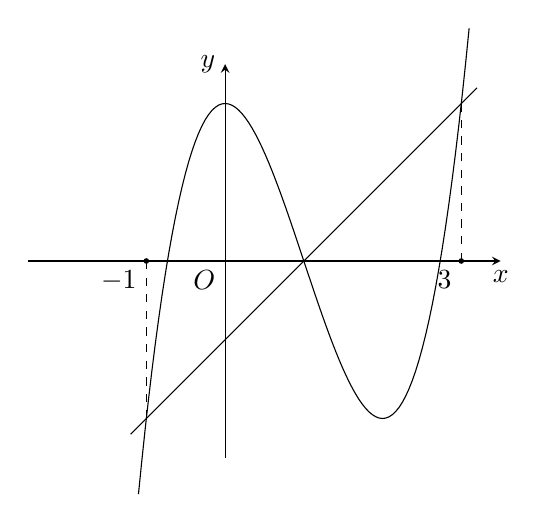
\begin{tikzpicture}
		\draw[-stealth] (-2.5,0)--(3.5,0)node[below]{$x$};
		\draw[-stealth] (0,-2.5)--(0,2.5)node[left]{$y$};
		\draw[samples=100,domain=-1.1:3.1]plot (\x,{(\x)^3-3*(\x)^2+2});
		\draw[samples=100,domain=-1.2:3.2]plot (\x,{(\x)-1});
		\foreach \i in{-1,3}{\draw[fill=black](\i,0)circle(0.8pt)node[below left]{$\i$};}
		\draw[dashed] (-1,0)--(-1,-2) (3,0)--(3,2) 
		(0,0)node[below left]{$O$}
		;
		\end{tikzpicture}
	\end{center}
	\choice
	{$-3$}
	{$-\dfrac{7}{3}$}
	{\True $-2$}
	{$-\dfrac{5}{2}$}
	\loigiai{
		\begin{itemize}
			\item Ta có: $f(x)=x-1 \Leftrightarrow \hoac{&x=-1\\&x=1\\&x=3\\}$.\\
			$f(x)$ là hàm bậc ba nên $f(x)-(x-1)=a(x+1)(x-1)(x-3)$\\
			Suy ra $f(x)=a(x+1)(x-1)(x-3)+x-1$.\\
			Ta có $f(0)=2\Leftrightarrow a=1$.\\
			Suy ra $f(x)=(x+1)(x-1)(x-3)+x-1$.
			\item $f(x)=0\Leftrightarrow \hoac{&x=1=x_2\\&(x+1)(x-3)+1=0&(2)\\}$.\\
			$x_1, x_3$ là các nghiệm của $(2)$ nên ta có $x_1x_3=-2$.\\
			Đường thẳng $y=\dfrac{5}{2}$ nên từ đồ thị ta có phương trình đã cho có $4$ nghiệm phân biệt.
		\end{itemize}
	}
\end{ex}
\begin{ex}%[2D1K5-4]
	Có bao nhiêu giá trị nguyên của tham số $m\in[-2018;2019]$ để đồ thị hàm số $y=x^3-3m x+3$ và đường thẳng $y=3x+1$ có duy nhất một điểm chung?
	\choice
	{$1$}
	{$2019$}
	{$4038$}
	{\True $2018$}
	\loigiai{
		Phương trình hoành độ giao điểm \\
		\centerline{
			$x^3-3mx+3=3x+1\Leftrightarrow x^3-3x+2=3mx\Leftrightarrow 3m=\dfrac{x^3-3x+2}{x}$. \tagEX{1}}\\
		Xét hàm $f(x)=\dfrac{x^3-3x+2}{x}=x^2-3+\dfrac{2}{x}$; $f'(x)=2x-\dfrac{2}{x^2}=\dfrac{2x^3-2}{x^2}$; $f'(x)=0\Leftrightarrow x=1$.\\
		Bảng biến thiên.
		\begin{center}
			
\begin{tikzpicture}
			\tkzTabInit[nocadre,lgt=1.2,espcl=3]{$x$/0.8,$f'(x)$/0.8,$f(x)$/2.5}{$-\infty$,$0$,$1$,$+\infty$}
			\tkzTabLine{,-,d,-,0,+,}
			\tkzTabVar{+/$+\infty$,-D+/$-\infty$/$+\infty$,-/$0$,+/$+\infty$}
			\end{tikzpicture}
		\end{center}
		Khi đó yêu cầu bài toán $\Leftrightarrow m<0$.\\ 
		Mà $m$ nguyên và $m\in[-2018;2019]$ nên có $2018$ giá trị thỏa mãn.
	}
\end{ex}
\begin{ex}%[2D1K5-4]
	Phương trình $x^3-6mx+5=5m^2$ có $3$ nghiệm phân biệt lập thành cấp số cộng khi
	\choice
	{$m=0$}
	{$m=-1\vee m=1$}
	{\True $m=1$}
	{$m \in \varnothing$}
	\loigiai{
		Phương trình đã cho tương đương: $x^3-6mx+5-5m^2=0$.\\
		Đặt $y=f(x)=x^3-6mx+5-5m^2$ có $f'(x)=3 x^2-6m$; $f''(x)=6x$.\\
		Phương trình đã cho có $3$ nghiệm phân biệt $\Leftrightarrow$ Hàm số $y=f(x)$ cắt trục hoành tại $3$ điểm phân biệt.\\
		$\Leftrightarrow f'(x)=0$ có $2$ nghiệm phân biệt $x_1$, $x_2$ thỏa mãn $f\left(x_1\right)\cdot f\left(x_2\right)<0$.\\
		$3$ nghiệm đó lập thành cấp số cộng nên $x_2-x_1=x_3-x_2$.\\
		Suy ra, $x_2$ là hoành độ của tâm đối xứng hay là nghiệm của $f''(x)=0$.\\
		Cho $f''(x)=0\Rightarrow 6x=0\Leftrightarrow x=0$.\\
		Với $x=0$ ta có: $5-5m^2=0\Leftrightarrow m=\pm 1$.\\
		Thử lại:
		\begin{itemize}
			\item Với $m=1$ thì ta có $x^3-6 x+5=5 \Leftrightarrow x\left(x^2-6\right)=0 \Leftrightarrow \hoac{&x=0\\&x=\pm \sqrt{6}\\}$.
			\item Với $m=-1$ thì ta có: $x^3+6x+5=5\Leftrightarrow x\left(x^2+6\right)=0\Leftrightarrow x=0$.
		\end{itemize}
	}
\end{ex}
\begin{ex}%[2D1K5-4]
	Tính tổng tất cả các giá trị của $m$ biết đồ thị hàm số $y=x^3+2mx^2+(m+3)x+4$ và đường thẳng $y=x+4$ cắt nhau tại ba điểm phân biệt $A(0;4)$, $B$, $C$ sao cho diện tích tam giác $IBC$ bằng $8\sqrt{2}$ với $I(1;3)$.
	\choice
	{$3$}
	{$8$}
	{\True $1$}
	{$5$}
	\loigiai{
		Gọi đồ thị hàm số $y=x^3+2mx^2+(m+3)x+4$ là $\left(C_m\right)$ và đồ thị hàm số $y=x+4$ là $(d)$.\\
		Phương trình hoành độ giao điểm của $\left(C_m\right)$ và $(d)$ là\\
		$x^3+2mx^2+(m+3)x+4=x+4\Leftrightarrow x^3+2mx^2+(m+2)x=0\quad (*) \Leftrightarrow \hoac{&x=0\\&x^2+2mx+m+2=0\\}$.\\
		Gọi $g(x)=x^2+2mx+m+2$.\\
		$(d)$ cắt $\left(C_m\right)$ tại ba điểm phân biệt $\Leftrightarrow$ phương trình $(*)$ có ba nghiệm phân biệt.\\
		$\Leftrightarrow$ phương trình $g(x)=0$ có hai nghiệm phân biệt khác $0$.\\
		$\Leftrightarrow \heva{&\Delta'_{g}>0\\&g(0)\ne 0\\}\Leftrightarrow \heva{&m^2-m-2>0\\&m+2\ne 0\\}\Leftrightarrow \heva{&\hoac{&m<-1\\
				&m>2\\}\\
			&m\ne -2\\}$ $(a)$.\\
		$x=0$ là hoành độ điểm $A$, hoành độ điểm $B$, $C$ là hai nghiệm $x_1$, $x_2$ của phương trình $g(x)=0$.\\
		$BC^2=\left(x_2-x_1\right)^2+\left[\left(x_2+4\right)-\left(x_1+4\right)\right]^2=2\left(x_2-x_1\right)^2$ (do $B$, $C$ thuộc đường thẳng $(d)$).\\
		Suy ra $BC^2=2\left[\left(x_2+x_1\right)^2-4 x_1 x_2\right]=8\left(m^2-m-2\right)$.\\
		Viết phương trình đường thẳng $(d)$ dưới dạng $x-y+4=0$, ta có
		$d(I,(d))=\dfrac{|1-3+4|}{\sqrt{2}}=\sqrt{2}$.\\
		$\begin{aligned}
		S_{IBC}=8\sqrt{2}\Leftrightarrow\dfrac{1}{2}BC\cdot d(I,(d))=8\sqrt{2}&\Leftrightarrow\dfrac{1}{4}BC^2\cdot[d(I,(d))]^2=128\\
		&\Leftrightarrow \dfrac{1}{4}8\left(m^2-m-2\right)\cdot 2=128 \\
		&\Leftrightarrow m^2-m-34=0\Leftrightarrow \hoac{&m=\dfrac{1+\sqrt{137}}{2}\\&m=\dfrac{1-\sqrt{137}}{2}} \\
		\end{aligned}$\\
		(thỏa điều kiện $(a)$).\\
		Vậy tổng tất cả các giá trị $m$ là $1$. 
	}
\end{ex}
\begin{ex}%[2D1K5-4]
	Có bao nhiêu giá trị nguyên của tham số $m\in[-2018;2019]$ để đồ thị hàm số $y=x^3-3mx+3$ và đường thẳng $y=3x+1$ có duy nhất một điểm chung?
	\choice
	{$1$}
	{$2019$}
	{$4038$}
	{\True $2018$}
	\loigiai{
		Phương trình hoành độ giao điểm: $x^3-3mx+3=3x+1\Leftrightarrow 3mx=x^3-3x+2$.\hfill (1)\\
		Dễ thấy $x=0$ không thỏa.\\
		$(1)\Leftrightarrow 3m=x^2-3+\dfrac{2}{x}=f(x)$.\\
		$f'(x)=2x-\dfrac{2}{x^2}=\dfrac{2x^3-2}{x^2}=0\Leftrightarrow x=1$.\\
		Bảng biến thiên:
		\begin{center}
			
\begin{tikzpicture}
			\tkzTabInit[nocadre,lgt=1.2,espcl=3]{$x$/0.8,$f'(x)$/0.8,$f(x)$/2.5}{$-\infty$,$0$,$1$,$+\infty$}
			\tkzTabLine{,-,d,-,0,+,}
			\tkzTabVar{+/$+\infty$,-D+/$-\infty$/$+\infty$,-/$0$,+/$+\infty$}
			\end{tikzpicture}
		\end{center}
		Đồ thị hàm số $y=x^3-3mx+3$ và đường thẳng $y=3x+1$ có duy nhất một điểm chung $\Leftrightarrow 3m<0\Leftrightarrow m<0$.\\
		Do $m \in \mathbb{Z}$ và $m\in[-2018;2019]$ nên có $2018$ giá trị.
	}
\end{ex}
\begin{ex}%[2D1K5-4]
	Đường thẳng $d$ có phương trình $y=x+4$ cắt đồ thị hàm số $y=x^3+2mx^2+(m+3)x+4$ tại $3$ điểm phân biệt $A(0;4)$, $B$ và $C$ sao cho diện tích của tam giác $MBC$ bằng $4$, với $M(1;3)$. Tìm tất cả các giá trị của $m$ thỏa mãn yêu cầu bài toán.
	\choice
	{\True $m=3$}
	{$m=2$ hoặc $m=3$}
	{$m=-2$ hoặc $m=-3$}
	{$m=-2$ hoặc $m=3$}
	\loigiai{
		Hoành độ giao điểm của hai đồ thị là nghiệm của phương trình $x^3+2mx^2+(m+3)x+4=x+4\Leftrightarrow x^3+2mx^2+(m+2)x=0 \Leftrightarrow \hoac{&x=0\\&x^2+2mx+(m-2)=0\quad (*)\\}$.\\
		Đường thẳng $d$ cắt đồ thị hàm số $(1)$ tại $3$ điểm phân biệt khi phương trình $(*)$ có hai nghiệm phân biệt khác $0 \Leftrightarrow \heva{&m^2-,-2>0\\&m+2\ne 0\\}\Leftrightarrow \heva{&\hoac{&m<-1\\
				&m>21\\}\\
			&m\ne -2\\}$.\\
		Giả sử $B\left(x_1;x_1+4\right)$; $C\left(x_2;x_2+4\right)$ với $x_1$; $x_2$ là nghiệm của phương trình $\left(^*\right)$ khi đó\\ \centerline{$BC=\sqrt{2\left(x_1-x_2\right)^2}=\sqrt{2\left(x_1+x_2\right)^2-8x_1\cdot x_2}=\sqrt{8m^2-8m-16}$.}\\ 
		Suy ra $S_{MBC}=\dfrac{1}{2}BC\cdot d(M, d)=\dfrac{1}{2}\cdot BC\cdot \dfrac{|1-3+4|}{\sqrt{2}}=4\Rightarrow BC=4\sqrt{2}$.\\
		Ta có $m^2-m-6=0\Leftrightarrow \hoac{&m=-2\\&m=3\\}$.\\
		Đối chiếu điều kiện ta có $m=3$.
	}
\end{ex}
\begin{ex}%[2D1K5-4]
	Tìm tất cả các giá trị thực của tham số $m$ để đường thẳng $y=-x+5$ cắt đồ thị hàm số $y=x^3+2mx^2+3(m-1)x+5$ tại $3$ diểm phân biệt.
	\choice
	{$\hoac{&m<1\\&m>2\\}$}
	{$\hoac{&\heva{&m\ne \dfrac{2}{3}\\
				&m\le 1\\}\\
			&m\ge 2\\}$}
	{\True $\hoac{&\heva{&m\ne \dfrac{2}{3}\\
				&m<1\\}\\
			&m>2\\}$}
	{$\hoac{&m\le 1\\&m\ge 2\\}$}
	\loigiai{
		Phương trình hoành độ giao điểm chung là $x^3+2mx^2+3(m-1) x+5=-x+5$.\\
		\centerline{$\Leftrightarrow x^3+2mx^2+(3m-2)x=0\Leftrightarrow \hoac{&x=0\\&x^2+2mx+3m-2=0\quad (1)}$.}\\
		Đường thẳng $y=-x+5$ cắt đồ thị hàm số $y=x^3+2mx^2+3(m-1)x+5$ tại $3$ điểm phân biệt.\\
		$\Leftrightarrow$ phương trình $(1)$ có hai nghiệm phân biệt khác $0$.\\
		$\Leftrightarrow \heva{&\Delta'=m^2-3m+2>0\\&3m-2\ne 0\\}\Leftrightarrow \heva{&\hoac{&m>2\\
				&m<1\\}\\
			&m\ne \dfrac{2}{3}\\}
		\Leftrightarrow \hoac{&\heva{&m\ne \dfrac{2}{3}\\
				&m<1\\}\\
			&m>2\\}$.
	}
\end{ex}
\begin{ex}%[2D1K5-4]
	Gọi $S$ là tập tất cả các giá trị thực của tham số $m$ để phương trình $2 x^3-3x^2=2 m+1$ có đúng hai nghiệm phân biệt. Tổng các phần tử của $S$ bằng
	\choice
	{$-\dfrac{1}{2}$}
	{\True $-\dfrac{3}{2}$}
	{$-\dfrac{5}{2}$}
	{$\dfrac{1}{2}$}
	\loigiai{
		Xét hàm số: $y=2 x^3-3x^2\Rightarrow y'=6x^2-6x\Rightarrow y'=0\Leftrightarrow x=0\vee x=1$.\\
		Bảng biến thiên:
		\begin{center}
			
\begin{tikzpicture}
			\tkzTabInit[nocadre,lgt=1.2,espcl=3]{$x$/0.8,$f'(x)$/0.8,$f(x)$/2.5}{$-\infty$,$0$,$1$,$+\infty$}
			\tkzTabLine{,+,0,-,0,+,}
			\tkzTabVar{-/$-\infty$,+/$0$,-/$-1$,+/$+\infty$}
			\end{tikzpicture}
		\end{center}
		Số nghiệm của phương trình đã cho bằng số giao điểm của hai đồ thị $\heva{&(C)\colon y=2x^3-3x^2\\&d\colon y=2m+1\\}$.\\
		Nhìn vào bảng biến thiên ta thấy: Phương trình đã cho có hai nghiệm phân biệt\\ 
		\centerline{$\Leftrightarrow \hoac{&2m+1=-1\\&2m+1=0\\}\Leftrightarrow \hoac{&m=-1\\&m=-\dfrac{1}{2}\\}\Rightarrow S=\left\{-1;-\dfrac{1}{2}\right\}$.}\\
		Vậy tổng các phần tử của $S$ bằng $-1+\left(-\dfrac{1}{2}\right)=\dfrac{-3}{2}$.
	}
\end{ex}
\begin{ex}%[2D1K5-4]
	Giá trị lớn nhất của $m$ để đường thẳng $(d)\colon y=x-m+1$ cắt đồ thị hàm số $y=x^3+2(m-2)x^2+(8-5m)x+m-5$ tại 3 điểm phân biệt có hoành độ $x_1$, $x_2$, $x_3$ thỏa mãn điều kiện $x_1^2+x_2^2+x_3^2=20$ là
	\choice
	{\True $3$}
	{$1$}
	{$0$}
	{$-\dfrac{3}{2}$}
	\loigiai{
		Hoành độ giao điểm của đường thẳng $(d)$ và đồ thị hàm số là nghiệm của phương trình\\
		$\begin{aligned}
		&x^3+2(m-2) x^2+(8-5 m) x+m-5=x-m+1 \\
		&\Leftrightarrow(x-2)\left[x^2+(2 m-2) x-m+3\right]=0 \Leftrightarrow \hoac{&x_3=2\\&x^2+(2m-2)x-m+3=0\quad (1)\\}
		\end{aligned}$\\
		Đường thẳng $(d)$ cắt đồ thị hàm số tại $3$ điểm phân biệt $\Leftrightarrow$ phương trình $(1)$ có hai nghiệm phân biệt $x_1$; $x_2$ khác $2\Leftrightarrow \heva{&\Delta'=(m-1)^2+(m-3)>0\\&4+(2m-2)\cdot 2-m+3\ne 0\\}\Leftrightarrow \heva{&\hoac{&m<-1\\
				&m>21\\}\\
			&m\ne -1\\}\Leftrightarrow \hoac{&m<-1\\&m>2\\}$ $(2)$.\\
		Khi đó, $\heva{&x_1+x_2=-(2m-2)\\&x_1x_2=-m+3\\}$.\\
		Theo giả thiết $x_1^2+x_2^2+x_3^2=20\Leftrightarrow\left(x_1+x_2\right)^2-2 x_1 x_2+x_3^2=20$.\\
		Vậy giá trị lớn nhất của $m$ thỏa mãn yêu cầu bài toán là $3$.
	}
\end{ex}
\begin{ex}%[2D1K5-4]
	Có bao nhiêu giá trị của $m$ để đồ thị hàm số $y=-2x^3-3m^2x^2+\left(m^3+2 m\right) x+2$ cắt trục hoành tại ba điểm phân biệt có hoành độ là ba số hạng liên tiếp của một cấp số nhân?
	\choice
	{$0$}
	{$1$}
	{\True $2$}
	{$3$}
	\loigiai{
		Hoành độ giao điểm của đồ thị với trục hoành là nghiệm của phương trình\\ 
		\centerline{$-2x^3-3m^2x^2+\left(m^3+2 m\right) x+2=0\quad (*)$.}\\
		Giả sử đồ thị cắt trục hoành tại $3$ điểm có hoành độ $x_1$, $x_2$, $x_3$.\\
		Khi đó\\
		\centerline{$y=-2\left(x-x_1\right)\left(x-x_2\right)\left(x-x_3\right)=-2x^3+2\left(x_1+x_2+x_3\right)x^2-2\left(x_1x_2+x_2x_3+x_3x_1\right)x+2x_1x_2x_3$.}\\
		Đồng nhất thức ta được\\
		$\heva{&2(x_1+x_2+x_3)=-3m^2\\&-2(x_1x_2+x_2x_3+x_3x_1)=m^3+2m\\&2x_1x_2x_3=2\\}\Leftrightarrow \heva{&x_1+x_2+x_3=-\dfrac{3m^2}{2}&(1)\\&x_1x_2+x_2x_3+x_3x_1=-\dfrac{m^3+2m}{2}&(2)\\&x_1x_2x_3=1&(3)\\}$.\\
		Vì $x_1$, $x_2$, $x_3$ lập thành cấp số nhân nên $x_1x_3=x_2^2$ $(4)$.\\
		Từ $(2)$ và $(3):x_2=1$. Thay vào phương trình $(*)$ rút ra được $\hoac{&m=0\\&m=1\\&m=2\\}$.\\
		Với $m=0 \Rightarrow$ phương trình $(*):-2x^3+2=0\Leftrightarrow x=1$ (không thỏa mãn).
		Với $m=1 \Rightarrow$ phương trình $(*):-2x^3-3x^2+3x+2=0\Leftrightarrow \hoac{&x_1=-2\\&x_2=1\\&x_3=-\dfrac{1}{2}\\}$ (thỏa mãn).\\
		Với $m=2\Rightarrow$ phương trình $(*): x^3+6x^2-6x-1=0\Leftrightarrow \hoac{&x_1=\dfrac{-7-\sqrt{45}}{2}\\&x_2=2\\&x_3=\dfrac{-7+\sqrt{45}}{2}}$ (thỏa mãn).\\
		Vậy có $2$ giá trị $m$ thỏa mãn.
	}
\end{ex}
\begin{ex}%[2D1K5-4]
	Tìm $m$ để đồ thị $(C)$ của $y=x^3-3x^2+4$ và đường thẳng $y=mx+m$ cắt nhau tại $3$ điểm phân biệt $A(-1;0)$, $B$, $C$ sao cho $\triangle OBC$ có diện tích bằng $64$.
	\choice
	{$m=14$}
	{$m=15$}
	{\True $m=16$}
	{$m=17$}
	\loigiai{
		\begin{itemize}
			\item \textbf{Cách 1:} $d(O, B C)=\dfrac{m}{\sqrt{m^2+1}}$.\\
			$\begin{aligned}
			BC&=\sqrt{\left(x_B-x_C\right)^2+\left(y_b-y_c\right)^2}=\sqrt{\left(m^2+1\right)\left(x_B-x_C\right)^2}\\
			&=\sqrt{\left(m^2+1\right)\left[\left(x_B+x_C\right)^2-4 x_B x_C\right]}=\sqrt{\left(m^2+1\right)4m}.\\
			\end{aligned}$\\
			Suy ra $S_{\triangle OBC}=\dfrac{1}{2}d(O, BC)\cdot BC=m\sqrt{m}=64\Leftrightarrow m=16$.
			\item \textbf{Cách 2:} Phương trình hoành độ giao điểm:\\
			$x^3-3x^2+4=m x+m \Leftrightarrow(x+1)(x^2-4 x+4-m)=0 \Leftrightarrow \hoac{&x=-1\\&(x-2)^2=m&(*)\\}$.\\
			Để $d$ cắt $(C)$ tại $3$ điểm phân biệt nên phương trình $(*)$ có $2$ nghiệm phân biệt khác $-1\Leftrightarrow \heva{&m>0\\&m\ne 9\\}$.\\
			$(*)\Leftrightarrow \hoac{&x=2-\sqrt{m}\Rightarrow B(2-\sqrt{m};3 m-m \sqrt{m})\\&x=2+\sqrt{m}\Rightarrow C(2+\sqrt{m};3 m+m \sqrt{m})\\}$.\\
			$\overrightarrow{OB}=(2-\sqrt{m};3m-m\sqrt{m})$, $\overrightarrow{OC}=(2+\sqrt{m};3m+m\sqrt{m})$.\\
			$\Rightarrow S_{\triangle OBC}=\dfrac{1}{2}\left|[\overrightarrow{OB}, \overrightarrow{OC}]\right|=m\sqrt{m}=64\Rightarrow m=16$.
		\end{itemize}
	}
\end{ex}
\begin{ex}%[2D1K5-4]
	Cho hàm số $y=x^3-8x^2+8x$ có đồ thị $(C)$ và hàm số $y=x^2+(8-a)x-b$ (với $a, b\in \mathbb{R}$) có đồ thị $(P)$. Biết đồ thị hàm số $(C)$ cắt $(P)$ tại ba điểm có hoành độ nằm trong $[-1;5]$. Khi $a$ đạt giá trị nhỏ nhất thì tích $ab$ bằng
	\choice
	{$-729$}
	{\True $375$}
	{$225$}
	{$-384$}
	\loigiai{
		\begin{itemize}
			\item \textbf{Cách 1:} Phương trình hoành độ giao điểm là $x^3-8x^2+8 x=x^2+(8-a)x-b\Leftrightarrow x^3-9x^2+ax+b=0$. \hfill (1)\\
			Gọi $m$, $n$, $p$ là $3$ nghiệm của phương trình $(1)$ ta có $\heva{&m+n+p=9\\&mn+np+pm=a\\&mnp=-b\\}$.\\
			Do $(C)$ cắt $(P)$ tại ba điểm có hoành độ nằm trong $[-1;5]$ nên\\
			$\heva{&(m+1)(n+1)(p+1)\geq 0\\&(5-m)(5-n)(5-p)\geq 0}\Leftrightarrow \heva{&mnp+(mn+np+pm)+(m+n+p)+1\geq 0\\&-mnp+5(mn+np+pm)-25(m+n+p)+125\geq 0\\}$.\\
			Cộng vế theo vế của hệ phương trình trên ta có $6(mn+np+pm)-24(m+n+p)-124\geq 0\Leftrightarrow mn+np+pm\geq 15\Rightarrow a\geq 15$.\\
			Dấu bằng xảy ra khi $\heva{&mnp\geq-25\\&mnp\leq-25\\}\Leftrightarrow mnp=-25 \Rightarrow b=25$.\\
			Vậy tích $ab=375$.
			\item \textbf{Cách 2:} Phương trình hoành độ giao điểm là\\
			$x^3-8x^2+8x=x^2+(8-a)x-b\Leftrightarrow x^3-9x^2+ax+b=0$.\hfill (1)\\
			Khi đó phương trình $(1)$ có $3$ nghiệm nằm trong $[-1;5]$.\\
			Đặt $f(x)=x^3-9x^2+ax+b$ suy ra $f'(x)=3x^2-18x+a$.\\
			Để phương trình $(1)$ có $3$ nghiệm nằm trong $[-1;5]$ thì $f'(x)=3x^2-18x+a=0$ có hai nghiệm phân biệt thuộc
			$[-1;5]\Leftrightarrow a=-3x^2+18x$ có hai nghiệm phân biệt thuộc $[-1;5]$.\\
			Xét hàm số $g(x)=-3x^2+18 x$ suy ra $g'(x)=-6x+18$, ta có $g'(x)=0\Leftrightarrow x=3$.\\
			Bảng biến thiên của $y=g(x)$
			\begin{center}
				
\begin{tikzpicture}
				\tkzTabInit[nocadre,lgt=1.2,espcl=3]{$x$/0.8,$g'(x)$/0.8,$g(x)$/2}{$-1$,$3$,$5$}
				\tkzTabLine{,+,0,-,}
				\tkzTabVar{-/$21$,+/$27$,-/$15$}
				\end{tikzpicture}
			\end{center}
			Từ BBT ta có $15\leq a<27$ suy ra giá trị nhỏ nhất của $a$ bằng $15$ khi $x=5$, khi đó $b=25$.\\
			Vậy tích $ab=375$.
		\end{itemize}
	}	
\end{ex}
\begin{ex}%[2D1K5-4]
	Có bao nhiêu giá trị nguyên của tham số $m$ để đường thẳng $y=-mx+m$ cắt đồ thị hàm số $y=x^3+mx^2+m$ tại $3$ điểm phân biêt có hoành độ $x_1$, $x_2$, $x_3$ thỏa mãn $-1<x_1+x_2+x_3<3 ?$
	\choice
	{$6$}
	{$5$}
	{\True $2$}
	{$3$}
	\loigiai{
		$(d)\colon y=-mx+m$, $(C)\colon y=x^3+mx^2+m$.\\
		Phương trình hoành độ giao điểm của $(d)$ và $(C): x^3+m x^2+m x=0(1)$.
		$\Leftrightarrow \heva{&x=0\\&x^2+m x+m=0&(2)\\}$.\\
		Gọi $x_1$, $x_2$ là $2$ nghiệm của phương trình $(2)$, $x_3=0$.\\
		$(1)$ có $3$ nghiệm phân biệt $\Leftrightarrow(2)$ có $2$ nghiệm $x_1$, $x_2$ phân biệt và khác $0$.\\
		$\Leftrightarrow \heva{&\Delta>0, \Delta=m^2-4 m\\&m\neq 0}\Leftrightarrow m\in(-\infty;0)\cup(4;+\infty)$.\\
		$(1)$ có $3$ nghiệm phân biệt $x_1$, $x_2$, $x_3$ thỏa $-1<x_1+x_2+x_3<3$, với $x_1+x_2=-m$, $x_3=0$.\\
		$\Leftrightarrow-1<-m<3$.\\
		$\Leftrightarrow-3<m<1$ mà $m\in(-\infty;0)\cup(4;+\infty)$, $m\in \mathbb{Z}$.\\
		$\Rightarrow m\in\left\{-2;-1\right\}$.\\ 
		Vậy có $2$ giá trị $m$ .
	}
\end{ex}
\begin{ex}%[2D1K5-4]
	Cho hàm số $y=x^3+2mx^2+(m+3)x+4\left(C_m\right)$. Tất cả các giá trị của tham số $m$ để đường thẳng $(d)\colon y=x+4$ cắt $\left(C_m\right)$ tại ba điểm phân biệt $A(0;4)$, $B$, $C$ sao cho tam giác $KBC$ có diện tích bằng $8\sqrt{2}$ với điểm $K(1;3)$ là:
	\choice
	{$m=\dfrac{1+\sqrt{137}}{2}$}
	{$m=\dfrac{\pm1+\sqrt{137}}{2}$}
	{\True $m=\dfrac{1\pm\sqrt{137}}{2}$}
	{$m=\dfrac{1-\sqrt{137}}{2}$}
	\loigiai{
		Phương trình hoành độ giao điểm của $\left(C_m\right)$ và $(d)$ là: $x^3+2mx^2+(m+3)x+4=x+4$.\hfill (1)
		$\begin{aligned}
		&\Leftrightarrow x^3+2mx^2+(m+2)x=0\\
		&\Leftrightarrow x\cdot\left[x^2+2 m x+(m+2)\right]=0 \\
		&\Leftrightarrow \hoac{&x=0\Rightarrow y=4\\&x^2+2mx+m+2=0&(2)}\\
		\end{aligned}$\\
		$(d)$ cắt $\left(C_m\right)$ tại ba điểm phân biệt.\\
		$\Leftrightarrow(1)$ có ba nghiệm phân biệt.\\
		$\Leftrightarrow(2)$ có hai nghiệm phân biệt khác $0$.\\
		$\Leftrightarrow \heva{&\Delta'>0\\&0^+2m\cdot 0+m+2\ne 0\\}\Leftrightarrow \heva{&m^2-m-2>0\\&m+2\ne 0\\}\Leftrightarrow \heva{&\hoac{&m>2\\
				&m<-1\\}\\
			&m\ne -2\\}\Leftrightarrow \hoac{&m>2\\
			&\heva{&m<-1\\
				&m\ne -2\\}\\}$.\\
		Khi đó, $(2)$ có hai nghiệm phân biệt $x_1$ và $x_2$ tương ứng cũng là hoành độ của $B$ và $C$.\\
		$\begin{aligned}
		&\Rightarrow B\left(x_1;x_1+4\right)\quad \text{và}\quad C\left(x_2;x_2+4\right).\\
		&\Rightarrow \overrightarrow{KB}=\left(x_1-1;x_2+1\right)\quad \text{và}\quad \overrightarrow{KC}=\left(x_2-1;x_2+1\right).\\
		\end{aligned}$\\
		$\Rightarrow S_{\triangle KBC}=\dfrac{\left|\left(x_1-1\right)\left(x_2+1\right)-\left(x_2-1\right)\left(x_1+1\right)\right|}{2}=\left|x_1-x_2\right|$.\\
		Theo đề bài: $S_{\triangle KBC}=8\sqrt{2}\Leftrightarrow\left|x_1-x_2\right|=8\sqrt{2}\Leftrightarrow\left(x_1-x_2\right)^2=128\Leftrightarrow S^2-4 P=128$.\\
		$\Leftrightarrow(-2m)^2-4(m+2)=128\Leftrightarrow m=\dfrac{1\pm \sqrt{137}}{2}$ (nhận).\\
		Vậy tất cả các giá trị $m$ thỏa đề là $m=\dfrac{1\pm \sqrt{137}}{2}$.
	}
\end{ex}
\begin{ex}%[2D1K5-4]
	Gọi $T$ là tập hợp tất cả các giá trị nguyên của tham số $m$ để phương trình $x^3-3x^2-m^3+3 m^2=0$ có ba nghiệm phân biệt. Tổng tất cả các phần tử của $T$ bằng
	\choice
	{\True $1$}
	{$5$}
	{$0$}
	{$3$}
	\loigiai{
		\begin{itemize}
			\item \textbf{Cách 1:} Ta có $x^3-3x^2-m^3+3m^2=0\Leftrightarrow x^3-3 x^2=m^3-3 m^2 \Leftrightarrow f(x)=f(m)$.\hfill (1)\\
			Xét hàm số $f(x)=x^3-3x^2$.\\
			$\begin{aligned}
			&f'(x)=3x^2-6x, f'(x)=0 \Leftrightarrow \hoac{&x=0\\&x=2\\}\\.
			&f(x)=0 \Leftrightarrow \hoac{&x=0\\&x=3\\}\\.
			&f(x)=-4 \Leftrightarrow \hoac{&x=2\\&x=-1\\}\\.
			\end{aligned}$\\
			\begin{center}
				
\begin{tikzpicture}
				\tkzTabInit[nocadre,lgt=1.2,espcl=2.5]{$x$/0.7,$f'(x)$/0.7,$f(x)$/2.5}{$-\infty$,$-1$,$0$,$2$,$3$,$+\infty$}
				\tkzTabLine{,,+,0,-,0,+,,}
				\tkzTabVar{-/$-\infty$,R,+/$0$,-/$-4$,R,+/$+\infty$}
				\tkzTabIma{1}{3}{2}{$-4$}
				\tkzTabIma{4}{6}{5}{$0$}
				\end{tikzpicture}
			\end{center}
			Dựa vào bảng biến thiên, suy ra $(1)$ có ba nghiệm phân biệt\\ \centerline{$\Leftrightarrow-4<f(m)<0\Leftrightarrow \heva{&-1<m<3\\&m\ne 0\\&m\ne 2\\}$.}\\
			Suy ra $T=\left\{1\right\}$. Vậy tổng tất cả các phần tử của $T$ bằng $1$.
			\item \textbf{Cách 2:} Ta có $x^3-3x^2-m^3+3m^2=0\Leftrightarrow\left(x^3-m^3\right)-3\left(x^2-m^2\right)=0\begin{aligned}
			&\Leftrightarrow(x-m)\left[x^2+(m-3) x+m^2-3 m\right]=0 \\
			&\Leftrightarrow \hoac{&x=m\\&x^2+(m-3)x+m^2-3m=0&(*)\\}
			\end{aligned}$\\
			Phương trình đã cho có $3$ nghiệm phân biệt $\Leftrightarrow(*)$ có hai nghiệm phân biệt, khác $m$\\
			$\begin{aligned}
			&\Leftrightarrow \heva{&\Delta=(m-3)^{2}-4(m^{2}-3m)>0\\&m^{2}+(m-3)m+m^{2}-3m\neq 0\\}\Leftrightarrow \heva{&(m-3)(-3m-3)>0\\&3m^2-6m\neq 0\\}\\
			&\Leftrightarrow \heva{&-1<m<3\\&m\ne 0\\&m\ne 2\\}\Rightarrow m=1\quad (\text{vì}\quad m\in \mathbb{Z})
			\end{aligned}$\\
			Suy ra $T=\left\{1\right\}$. Vậy tổng tất cả các phần tử của $T$ bằng $1$.
		\end{itemize}
	}
\end{ex}
\begin{ex}%[2D1K5-4]
	Cho đồ thị hàm số $f(x)=x^3+bx^2+c x+d$ cắt trục hoành tại 3 điểm phân biệt có hoành độ $x_1$, $x_2$, $x_3$. Tính giá trị của biểu thức $P=\dfrac{1}{f'\left(x_1\right)}+\dfrac{1}{f'\left(x_2\right)}+\dfrac{1}{f'\left(x_3\right)}$.
	\choice
	{$P=3+2 b+c$}
	{\True $P=0$}
	{$P=b+c+d$}
	{$P=\dfrac{1}{2 b}+\dfrac{1}{c}$}
	\loigiai{
		Vì $x_1$, $x_2$, $x_3$ là ba nghiệm của phương trình bậc ba $f(x)=0\Rightarrow f(x)=\left(x-x_1\right)\left(x-x_2\right)\left(x-x_3\right)$.\\
		Ta có $f'(x)=\left(x-x_1\right)\left(x-x_2\right)+\left(x-x_2\right)\left(x-x_3\right)+\left(x-x_1\right)\left(x-x_3\right)$.\\
		Khi đó $\heva{&f'(x_1)=(x_1-x_2)(x_1-x_3)\\&f'(x_2)=(x_2-x_3)(x_2-x_1)\\&f'(x_3)=(x_3-x_1)(x_3-x_2)}$.\\
		Suy ra $\begin{aligned}[t]
		P&=\dfrac{1}{\left(x_1-x_2\right)\left(x_1-x_3\right)}+\dfrac{1}{\left(x_2-x_3\right)\left(x_2-x_1\right)}+\dfrac{1}{\left(x_3-x_1\right)\left(x_3-x_2\right)}\\
		&=\dfrac{\left(x_2-x_3\right)-\left(x_1-x_3\right)+\left(x_1-x_2\right)}{\left(x_1-x_2\right)\left(x_1-x_3\right)\left(x_2-x_3\right)}=0.\\
		\end{aligned}$
	}
\end{ex}
\begin{ex}%[2D1K5-4]
	Cho hàm số bậc ba $y=f(x)$ có đồ thị đi qua điểm $A(1;1)$, $B(2;4)$, $C(3;9)$. Các đường thẳng $AB$, $AC$, $BC$ lại cắt đồ thị lần lượt tại các điểm $M$, $N$, $P$ ($M$ khác $A$ và $B$, $N$ khác $A$ và $C, P$ khác $B$ và $C$. Biết rằng tổng các hoành độ của $M$, $N$, $P$ bằng $5$, giá trị của $f(0)$ là
	\choice
	{$-6$}
	{\True $-18$}
	{$18$}
	{$6$}
	\loigiai{
		Từ giả thuyết bài toán ta giả sử $f(x)=a(x-1)(x-2)(x-3)+x^2(a\neq 0)$.\\
		Ta có: $AB\colon y=3x-2$, $AC\colon y=4x-3$, $BC\colon y=5x-6$.\\
		Khi đó hoành độ của $M$ là nghiệm của phương trình:\\ $a\left(x_M-1\right)\left(x_M-2\right)\left(x_M-3\right)+x_M^2=3 x_M-2 \Leftrightarrow a\left(x_M-1\right)\left(x_M-2\right)\left(x_M-3\right)+\left(x_M-1\right)\left(x_M-2\right)=0$.\\
		$\Leftrightarrow a\left(x_M-3\right)+1=0 \Leftrightarrow x_M=3-\dfrac{1}{a}$.\\
		Hoành độ của $N$ là nghiệm của phương trình:\\ 
		$a\left(x_N-1\right)\left(x_N-2\right)\left(x_N-3\right)+x_N^2=4 x_N-3 \Leftrightarrow a\left(x_N-1\right)\left(x_N-2\right)\left(x_N-3\right)+\left(x_N-1\right)\left(x_N-3\right)=0$.\\
		$\Leftrightarrow a\left(x_N-2\right)+1=0 \Leftrightarrow x_N=2-\dfrac{1}{a}$.\\
		Hoành độ của $P$ là nghiệm của phương trình:\\ 
		$a\left(x_P-1\right)\left(x_P-2\right)\left(x_P-3\right)+x_P^2=5 x_P-6 \Leftrightarrow a\left(x_P-1\right)\left(x_P-2\right)\left(x_P-3\right)+\left(x_P-2\right)\left(x_P-3\right)=0$.\\
		$\Leftrightarrow a\left(x_P-1\right)+1=0 \Leftrightarrow x_P=1-\dfrac{1}{a}$.\\
		Từ giả thuyết ta có $x_M+x_N+x_P=5\Leftrightarrow6-\dfrac{3}{a}=5\Leftrightarrow a=3$.\\
		Do đó: $f(x)=3(x-1)(x-2)(x-3)+x^2$.\\
		Vậy $f(0)=-18$.
	}
\end{ex}
\begin{ex}%[2D1K5-4]
	Tìm giá trị thực của tham số $m$ để đồ thị hàm số $y=x^3-3x^2+2$ cắt đường thẳng $d\colon y=m(x-1)$ tại ba điểm phân biệt có hoành độ $x_1$, $x_2$, $x_3$ thỏa mãn $x_1^2+x_2^2+x_2^2>5$.
	\choice
	{$m\geq-3$}
	{$m\geq-2$}
	{$m>-3$}
	{\True $m>-2$}
	\loigiai{
		Phương trình hoành độ giao điểm:\\
		$\begin{aligned}
		x^3-3 x^2+2=m(x-1)&\Leftrightarrow x^3-3 x^2-m x+m+2=0\\
		&\Leftrightarrow(x-1)\left(x^2-2 x-m-2\right)=0 \Leftrightarrow \hoac{&x_1=1\\&g(x)=x^2-2 x-(m+2)=0&(*)}\\
		\end{aligned}$\\
		Để hai đồ thị cắt nhau tại ba điểm phân biệt thì phương trình $(*)$ phải có hai nghiệm phân biệt khác $1\Leftrightarrow \heva{&\Delta'>0\\&g(1)\ne 0\\}\Leftrightarrow \heva{&1^2+(m+2)>0\\&1-2-m-2\ne 0\\}\Leftrightarrow \heva{&m>-3\\&m\ne -3\\}\Leftrightarrow m>-3$.\\
		Gọi $x_2$, $x_3$ là hai nghiệm phương trình $(*)$.\\
		Theo định lý Viét ta có $\heva{&x_2+x_3=2\\&x_2\cdot x_3=-(m+2)\\}$.\\
		Theo bài ta có $x_1^2+x_2^2+x_3^2>5\Leftrightarrow 1+x_2^2+x_3^2>5\Leftrightarrow x_2^2+x_3^2>4$.\\
		$\Leftrightarrow\left(x_2+x_3\right)^2-2x_2x_3>4\Leftrightarrow 4+2(m+2)>4\Leftrightarrow m>-2$.\\
		So sánh với điều kiện ở trên suy ra $m>-2$.\\
		Kết luận: $m>-2$ thỏa mãn yêu cầu bài toán
	}
\end{ex}
\begin{ex}%[2D1K5-4]
	Gọi $S$ là tập tất cả các giá trị của tham số $m$ để đồ thị hàm số $y=x^3+3x^2-9x+2 m+1$ và trục $Ox$ có đúng hai điểm chung phân biệt. Tính tổng $T$ của các phần tử thuộc tập $S$
	\choice
	{$T=-10$}
	{$T=10$}
	{\True $T=-12$}
	{$T=12$}
	\loigiai{
		Hoành độ giao điểm của đồ thị hàm số $y=x^3+3x^2-9x+2 m+1$ và trục $O x$ là nghiệm của phương trình : $x^3+3x^2-9x+2m+1=0 \Leftrightarrow-x^3-3x^2+9x=2m+1$.\\
		Xét hàm số $f(x)=-x^3-3 x^2+9 x$.\\
		Tập xác định: $\mathscr{D}=\mathbb{R}$.\\
		$f'(x)=-3x^2-6x+9$, $f'(x)=0\Leftrightarrow-3x^2-6 x+9=0\Leftrightarrow \hoac{&x=1\\&x=-3\\}$.\\
		Bảng biến thiên:
		\begin{center}
			
\begin{tikzpicture}
			\tkzTabInit[nocadre,lgt=1.2,espcl=3]{$x$/0.8,$f'(x)$/0.8,$f(x)$/2.5}{$-\infty$,$-3$,$1$,$+\infty$}
			\tkzTabLine{,-,0,+,0,-,}
			\tkzTabVar{+/$+\infty$,-/$-27$,+/$5$,-/$-\infty$}
			\end{tikzpicture}
		\end{center}
		Đồ thị hàm số $y=x^3+3x^2-9x+2 m+1$ cắt trục $Ox$ tại hai điểm phân biệt khi và chỉ khi đường thẳng $y=2m+1$ cắt đồ thị hàm số $f(x)=-x^3-3x^2+9x$ tại hai điểm phân biệt.\\
		Từ bảng biến thiên suy ra: $\hoac{&2m+1=5\\&2m+1=-27\\}\Leftrightarrow \hoac{&m=2\\&m=-14\\}\Rightarrow S=\left\{-14;2\right\}$.\\
		Tổng của các phần tử thuộc tập $S$ là: $T=-14+2=-12$.
	}
\end{ex}
\begin{ex}%[2D1K5-4]
	Gọi $m_0$ là số thực sao cho phương trình $\left|x^3-12x\right|=m_0$ có ba nghiệm dương phân biệt $x_1$; $x_2$; $x_3$ thỏa mãn $x_1+x_2+x_3=1+4\sqrt{3}$. Biết rằng $m_0$ có dạng $a \sqrt{3}+b$ với $a$; $b$ là các số hữu tỷ. Tính $4a^2+8b$.
	\choice
	{\True $106$}
	{$115$}
	{$113$}
	{$101$}
	\loigiai{
		Vẽ đồ thị hàm số $y=\left|x^3-12x\right|$.
		\begin{center}
			\begin{tikzpicture}[y=0.4cm]
			\draw[-stealth] (-4.5,0)--(4.5,0)node[below]{$x$};
			\draw[-stealth] (0,-0.5)--(0,20)node[left]{$y$};
			\draw[samples=100,domain=-4:-3.46] plot (\x,{-(\x)^3+12*(\x)});
			\draw[samples=100,domain=0:3.46] plot (\x,{-(\x)^3+12*(\x)});
			\draw[samples=100,domain=-3.46:0] plot (\x,{(\x)^3-12*(\x)});
			\draw[samples=100,domain=3.46:4] plot (\x,{(\x)^3-12*(\x)});
			\draw[dashed] (-2,0)--(-2,16)--(0,16)node[above left]{$16$}--(2,16)--(2,0);
			\end{tikzpicture}
		\end{center}
		Do đó với mọi $m\in(0;16)$ thì phương trình đã cho luôn có ba nghiệm dương phân biệt $x_1$; $x_2$; $x_3$ $\left(x_1<x_2<x_3\right)$ thỏa mãn: $\heva{&-x_1^3+12 x_1=m_0\\&-x_2^3+12 x_2=m_0\\&x_3^3-12x_3=m_0}\Leftrightarrow \heva{&\left(-x_1\right)^3-12\left(-x_1\right)-m_0=0\\&\left(-x_2\right)^3-12\left(-x_2\right)-m_0=0\\&x_3^3-12x_3-m_0=0\\}$.\\
		$\Rightarrow-x_1$; $-x_2$; $x_3$ là ba nghiệm của phương trình $x^3-12x-m_0=0$.\\
		$\Rightarrow-x_1-x_2+x_3=0\Rightarrow x_3=x_1+x_2$.\\
		Mà $x_1+x_2+x_3=1+4 \sqrt{3}\Rightarrow x_3=\dfrac{1+4\sqrt{3}}{2}$ 
		$\Rightarrow m_0=\left(\dfrac{1+4\sqrt{3}}{2}\right)^3-12\left(\dfrac{1+4\sqrt{3}}{2}\right)=\dfrac{3\sqrt{3}}{2}+\dfrac{97}{8}$.\\ $\Rightarrow a=\dfrac{3}{2}; b=\dfrac{97}{8}\Rightarrow 4a^2+8 b=106$.
	}	
\end{ex}
\begin{ex}%[2D1K5-4]
	Cho hàm số $y=x^3+3x^2-3mx+m-1$. Biết rằng hình phẳng giới hạn bởi đồ thị hàm số và trục $Ox$ có diện tích phần nằm phía trên trục $Ox$ và phần nằm dưới trục $Ox$ bằng nhau. Giá trị của $m$ là?
	\choice
	{$-\dfrac{2}{3}$}
	{$\dfrac{2}{3}$}
	{$1$}
	{\True $-\dfrac{1}{4}$}
	\loigiai{
		Ta có $y'=3x^2+6x-3m$ và $y''=6x+6$, $y''=0\Leftrightarrow x=-1$, $y(-1)=1+4m\Rightarrow U(-1;1+4 m)$.\\
		Từ giả thiết suy ra hàm số có hai điểm cực trị và điểm uốn nằm trên trục hoành, nên $1+4m=0\Leftrightarrow m=-\dfrac{1}{4}$.
	}
\end{ex}
\begin{ex}%[2D1K5-4]
	Số giá trị nguyên của tham số $m\in[-2020;2021]$ để đường thẳng $y=3mx+1$ cắt đồ thị hàm số $y=x^3-3x+3$ tại ba điểm phân biệt là
	\choice
	{$1$}
	{\True $2021$}
	{$670$}
	{$2020$}
	\loigiai{
		\begin{itemize}
			\item Phương trình hoành độ giao điểm của đồ thị $y=x^3-3x+3$ và đường thẳng $y=3mx+1$ là $x^3-3x+3=3mx+1\Leftrightarrow x^3+2=3x(m+1)$.\hfill (1)\\
			Nếu $x=0$ thì $(1)$ không thỏa mãn.\\
			Nếu $x\neq 0$ ta có $(1)\Leftrightarrow \dfrac{x^3+2}{x}=3(m+1)$.
			\item Xét hàm số $g(x)=\dfrac{x^3+2}{x}$ với $x\in \mathbb{R}\backslash\left\{0\right\}$.\\
			Ta có $g'(x)=\dfrac{2x^3-2}{x^2}$, $\forall x\in\mathbb{R}\backslash\left\{0\right\}$.\\
			$g'(x)=0\Leftrightarrow x=1$.\\
			Bảng biến thiên của hàm số $g(x)=\dfrac{x^3+2}{x}$ với $x\in \mathbb{R}\backslash\left\{0\right\}$.
			\begin{center}
				
\begin{tikzpicture}
				\tkzTabInit[nocadre,lgt=1.2,espcl=3]{$x$/0.8,$g'(x)$/0.8,$g(x)$/2.5}{$-\infty$,$0$,$1$,$+\infty$}
				\tkzTabLine{,-,d,-,0,+,}
				\tkzTabVar{+/$+\infty$,-D+/$-\infty$/$+\infty$,-/$3$,+/$+\infty$}
				\end{tikzpicture}
			\end{center}
			\item Dựa vào bảng biến thiên ta thấy đồ thị hàm số đã cho cắt đường thẳng $y=3mx+1$ tại $3$ điểm phân biệt $\Leftrightarrow3(m+1)>3\Leftrightarrow m+1>1 \Leftrightarrow m\in(0;+\infty)$.\\
			Kết hợp với điều kiện $m\in[-2020;2021]$ ta được $m\in(0;2021]$.\\
			Do $m\in\mathbb{Z}\Rightarrow m\in\left\{1;2;3;\ldots;2021\right\}$
		\end{itemize}
	}
\end{ex}
\begin{dang}{Bài toán tương giao của đường thẳng với đồ thị hàm số nhất biến (chứa tham số)}
\end{dang}
\begin{ex} %[SGD-ĐT Ninh Bình 2020]% Lê Xuân Hòa]%[2D1K5-4]
	Có tất cả bao nhiêu giá trị nguyên thuộc đoạn $\left[ -2020; 2020\right]$  của tham số $m$  để đường thẳng  $y=x+m$ cắt đồ thị hàm số $y=\dfrac{2x-3}{x-1}$   tại hai điểm phân biệt?
	\choice
	{\True $4036$}
	{$4040$}
	{$4038$}
	{$4034$}
	\loigiai{
		Ta có phương trình hoành dộ giao điểm của đường thẳng $y=x +m$ và đường cong $y= \dfrac{2x -3}{x-1}$ là 
		$x - m = \dfrac{2x-3}{x-1}\Leftrightarrow g(x) = x^2 +(m-3)x -m+3 =0, x\ne 1$\quad $(1)$ có $\Delta = (m-3)^2 -4(-m+3) = m^2 -2m -3$\\
		Để đường thẳng $y=x+m$ cắt đồ thị hàm số $y=\dfrac{2x-3}{x-1}$ tại hai điểm phân biệt thì $(1)$ có hai nghiệm phân biệt khác $1$ $\Leftrightarrow\heva{&\Delta > 0\\& g(1)\ne 0}\Leftrightarrow \heva{&m^2 -2m -3>0\\& 1\ne 0}\Leftrightarrow \hoac{& m<-1\\& m>3}$\\
		Kết hợp giả thiết: $\heva{&-2020 \le m \le 2020\\& m\in\mathbb{Z}\\& m<-1; m>3}
		\Leftrightarrow\heva{&m\in\mathbb{Z}\\&\hoac{&-2020 \le m<-1\\&3<m\le 2020}}$. \\
		Trường hợp $1$: $\heva{m\in\mathbb{Z}\\& -2020 \le m<-1}\Rightarrow $ có $\dfrac{-2-(-2020)}{1}+1 = 2019$ giá trị nguyên $m$.\\
		Trường hợp $2$:  $\heva{&m\in\mathbb{Z}\\& 3 \le m<2020}\Rightarrow $ có $\dfrac{2020-4}{1}+1 = 2017$ giá trị nguyên $m$.\\
		Vậy có tất cả $2019 + 2017 = 4036$ giá trị nguyên của tham số $m$.
	}
\end{ex}
%2
\begin{ex}%[ĐHQG TPHCM 2019, Lê Xuân Hòa]%[2D1K5-4]
	Đường thẳng  $y=x+2m$ cắt đồ thị hàm số $y=\dfrac{x-3}{x-1}$   tại hai điểm phân biệt khi và chỉ khi?
	\choice
	{\True $\hoac{&m<-1\\&m>3}$}
	{$\hoac{&m\le -1\\&m\ge 3}$}
	{$\hoac{&m<-3\\&m>1}$}
	{$-3<m<1$}
	\loigiai{
		Ta có phương trình hoành dộ giao điểm của đường thẳng $y=x +2m$ và đường cong $y= \dfrac{x -3}{x-1}$ là 
		$x +2m = \dfrac{x-3}{x-1}\Leftrightarrow g(x) = x^2 +2mx +2m+3 =0, x\ne 1$\quad $(1)$ có $\Delta '= (m)^2 -(2m+3) = m^2 +2m +3$\\
		Để đường thẳng $y=x+m$ cắt đồ thị hàm số $y=\dfrac{2x-3}{x-1}$ tại hai điểm phân biệt thì $(1)$ có hai nghiệm phân biệt khác $1$ $\Leftrightarrow\heva{&\Delta > 0\\& g(1)\ne 0}\Leftrightarrow \heva{&m^2 +2m+3>0\\& -4\ne 0}\Leftrightarrow \hoac{& m<-1\\& m>3}$\\
		Vậy tập hợp các giá trị của tham số $m$ là   $\hoac{&m<-1\\&m>3}$.
	}
\end{ex}
%3
\begin{ex}%[Gia Lai 2019, Lê Xuân Hòa]%[2D1K5-4]
	Tìm tất cả các giá trị thực của tham số $m$ để dường thẳng  $y=2x+m$ cắt đồ thị hàm số $y=\dfrac{x+3}{x+1}$   tại hai điểm phân biệt?
	\choice
	{\True $m\in\left( -\infty ; +\infty\right)$}
	{$m\in\left( -1 ; +\infty\right)$}
	{$m\in\left( -2 ; 4 \right)$}
	{$m\in\left( -\infty ; -2\right)$}
	\loigiai{
		Ta có phương trình hoành dộ giao điểm của đường thẳng $y=x +2m$ và đường cong $y= \dfrac{x -3}{x-1}$ là 
		$x +2m = \dfrac{x-3}{x-1}\Leftrightarrow g(x) = x^2 +2mx +2m+3 =0, x\ne 1$\quad $(1)$ có $\Delta '= (m)^2 -(2m+3) = m^2 +2m +3$\\
		Để đường thẳng $y=x+m$ cắt đồ thị hàm số $y=\dfrac{2x-3}{x-1}$ tại hai điểm phân biệt thì $(1)$ có hai nghiệm phân biệt khác $1$ $\Leftrightarrow\heva{&\Delta > 0\\& g(1)\ne 0}\Leftrightarrow \heva{&m^2 +2m+3>0\\& -4\ne 0}\Leftrightarrow \hoac{& m<-1\\& m>3}$\\
		Vậy tập hợp các giá trị của tham số $m$ là   $\hoac{&m<-1\\&m>3}$.
	}
\end{ex}


\begin{ex}%[Lê Xuân Hòa]%[2D1K5-4]
	Gọi $A$  và $B$  là hai điểm thuộc hai nhánh khác nhau của đồ thị hàm số $y=\dfrac{x}{x-2}$ . Khi đó độ dài đoạn $AB$  ngắn nhất bằng
	\choice
	{$4\sqrt{2}$}
	{\True $4$}
	{$2\sqrt{2}$}
	{$\sqrt{2}$}
	\loigiai{
		Gọi $A\left( a; \dfrac{a}{a-2}\right)$ và $B\left( b; \dfrac{b}{b-2}\right)$ là hai điểm thuộc hai nhánh của đồ thị hàm số $y=\dfrac{x}{x-2}$, $(a<2<b)$.\\
		Ta có $\overrightarrow{AB}=\left( b-a; \dfrac{b-a}{(b-2)(a-2)}\right)$.\\
		Áp dụng BĐT Côsi, ta có $(b-2)(a-2)\le \dfrac{(b-a)^2}{4}$.\\
		Suy ra $AB^2 = (b-a)^2 +\dfrac{(b-a)^2}{\left[(b-2)(a-2)\right]^2} \ge (b-a)^2 +\dfrac{64}{(b-a)^2}\ge 16$. Suy ra $AB\ge 4$. Dấu bằng xảy ra khi và chỉ khi $a=2-\sqrt{2}$ à $b=2+\sqrt{2}$.\\
		Vậy $AB=4$
	}
\end{ex}

\begin{ex}%[Lê Xuân Hòa]%[2D1K5-4]
	Cho hàm số  $y=\dfrac{x}{x-1}$ và đường thẳng $d\colon y = -x +m$  . Gọi $S$   là tập các số thực $m$  để đường thẳng $d$  cắt đồ thị  $\mathrm{(C)}$ tại hai điểm phân biệt  $A$, $B$ sao cho tam giác $OAB$  ( $O$ là gốc tọa độ) có bán kính đường tròn ngoại tiếp bằng  $2\sqrt{2}$. Tổng các phần tử của  $S$ bằng
	\choice
	{\True $4$}
	{$3$}
	{$0$}
	{$8$}
	\loigiai{
		Xét phương trình $\dfrac{x}{x-1}=-x+m \Leftrightarrow x^2 -mx +m = 0 \quad (1)$, $x\ne 1$.\\b
		Đồ thị $\mathrm{(C)}$ và đường thẳng $d$ cắt nhau tại hai điểm phân biệt $A$ và $B$ khi và chỉ khi phương trình $(1)$ có hai nghiệm phân biệt $x\ne 1$ $\Leftrightarrow \Delta = m^2 -4m \ge \Leftrightarrow m < 0; m > 4$.\\
		Khi đó hai giao điểm là $A\left( x_1; -x_1 + m\right)$, $B\left( x_2; -x_2+ m\right)$\\
		Ta có $OA = \sqrt{m^2 - 2m}$; $OB = \sqrt{m^2 - 2m}$; $AB = \sqrt{2(m^2 - 4m)}$; $\mathrm{d}(O;d) =\dfrac{|m|}{\sqrt{2}}$.\\
		Khi đó $S_{\text{OAB}}=\dfrac{1}{2}AB\cdot \mathrm{d}(O,d) = \dfrac{1}{2}\cdot \dfrac{|m|}{\sqrt{2}}\sqrt{2(m^2-4m)}=\dfrac{(m^2-2m)\sqrt{2(m^2-4m)}}{4\cdot 2\sqrt{2}}$\\
		$\Leftrightarrow m^2 -2m = 4|m| \Leftrightarrow \hoac{&m=0(\text{loại})\\& m=6(\text{nhận})\\& m=-2(\text{nhận})}$.\\
		Vậy tổng các phần tử của $S$ bằng $4$.
	}
\end{ex}


\begin{ex}%[Lê Xuân Hòa]%[2D1K5-4]
	Đô thị hàm số $y=\dfrac{2x-1}{1-x}$ có đồ thị $\mathrm{(C)}$ và đường thẳng $d\colon y = x + m$. Tìm tất cả các giá trị của tham số $m$ để đường thẳng $d$ cắt đồ thị $\mathrm{(C)}$ tại $2$ điểm phân biệt.
	\choice
	{$m>-1$}
	{$-5<m<-1$}
	{$m<-5$}
	{\True $m<-5; m>-1$}
	\loigiai{
		Hàm số $y=\dfrac{2x-1}{1-x}$ có tập xác định $\mathscr{D}=\mathbb{R}\setminus \left\{ 1\right\}$.\\
		Phương trình hoành độ giao điểm của hai  đường $\dfrac{2x-1}{1-x}=x+m \Leftrightarrow x^2 +(m+1)x -(m+1) = 0, x\ne 1$  \quad $(1)$.\\
		Đường thẳng $d$ cắt đồ thị hàm số tại hai điểm phân biệt $\Leftrightarrow $ phương trình $(1)$ có hai nghiệm phân biệt khác $1$.\\
		$\Leftrightarrow \heva{&\Delta > 0\\& 1^1 + (m+1) -(m+1) \ne 0}\Leftrightarrow \heva{& m^2 +6m +5 > 0\\& 1\ne 0}\Leftrightarrow m<-5; m > -1$
	}
\end{ex}


\begin{ex}%[Lê Xuân Hòa]%[2D1K5-4]
	Cho hàm số $y=\dfrac{x+3}{x+1}$  có đồ thị $\mathrm{(C)}$  và đường thẳng $d\colon y = x -m$  , với  $m$ là tham số thực. Biết rằng đường thẳng  $d$ cắt $\mathrm{(C)}$  tại hai điểm phân biệt  $A$ và  $B$ sao cho điểm  $G(2; -2)$ là trọng tâm của tam giác  $OAB$ (  $O$ là gốc toạ độ). Giá trị của $m$  bằng
	\choice
	{\True $6$}
	{$3$}
	{$-9$}
	{$5$}
	\loigiai{
		Hàm số $y=\dfrac{x+3}{x+1}$ có $y'=\dfrac{-2}{(x+1)^2}$, $\forall x\mathscr{D}$ và đường thẳng $d$ có hệ số $a=1> 0$ nên $d$ luôn cắt $\mathrm{(C)}$ tại hai điểm phân biệt $A(x_A; y_A$ và $B(x_B; y_B)$ với mọi giá trị của tham số $m$.\\
		Phương trình hoành độ giao điểm của $d$ và $\mathrm{(C)}$ là $\dfrac{x+3}{x+1}=x-m \Leftrightarrow x^2 -mx -m -3 =0$, $x\ne -1$.\\
		Suy ra $x_A$, $x_B$ là nghiệm phương trình $x^2 -mx - m -3 =0$.\\
		Theo định lí Vi-et, ta có $x_A + x_B = m$.\\
		Mặt khác, $G(2;-2)$ là trọng tâm của tam giác $OAB$ nên $x_A + x_B + x_O = 3x_G \Leftrightarrow x_A + x_B = 6 \Leftrightarrow m =6$.\\
		Vậy $m=6$ thỏa yêu cầu bài toán.
	}
\end{ex}


\begin{ex}%[Lê Xuân Hòa]%[2D1K5-4]
	Cho hàm số $y=\dfrac{3x-2m}{mx+1}$  với $m$  là tham số. Biết rằng với mọi  $m\ne 0$  đồ thị hàm số luôn cắt đường thẳng $d\colon y = 3x -3m$  tại hai điểm phân biệt $A$, $B$   Tích tất cả các giá trị của $m$  tìm được để đường thẳng $d$  cắt các trục $Ox$, $Oy$   lần lượt tại  $C$, $D$  sao cho diện tích $\Delta OAB$  bằng $2$ lần diện tích $\Delta OCD$  bằng
	\choice
	{\True $-\dfrac{4}{9}$}
	{$-4$}
	{$-1$}
	{$0$}
	\loigiai{
		Phương trình hoành độ giao điểm của hai đường $\dfrac{3x-2m}{mx+1}=3x-3m \Leftrightarrow 3x^2 - 3mx -1 = 0$\quad $(*)$\\
		Gọi tọa độ các giao điẻm của $d$ với đồ thị hàm số đã cho là $A(x_1; 3x_1-3m)$, $B(x_2; 3x_2-3m)$.\\
		Tọa độ các điểm $C(m;0)$, $D(0; -3m)$. Gọi $h =\mathrm{d}(O,d)$, suy ra $h$ là chiều cao của các tam giác $OAB$ và $OCD$.\\
		Theo giả thiết $S_{OAB}=2S_{OCD}\Leftrightarrow \dfrac{1}{2}AB\cdot h = 2\cdot\dfrac{1}{2}CD\cdot h \Leftrightarrow AB =2CD \Leftrightarrow AB^2 = 4CD^2$
		\begin{align*}
			\Leftrightarrow & (x_1-x_2)^2 + \left[ 3 (x_1 - x_2)\right]^2 = 4\left[ m^2 +(-3m)^2\right]\\\ \Leftrightarrow & (x_1 +x_2)^2 -4x_1x_2 =4m^2\\
			\Leftrightarrow & m^2 +\dfrac{4}{3}=4m^2 \Leftrightarrow m^2 =\dfrac{4}{9}\Leftrightarrow m=\pm \dfrac{2}{3}.
		\end{align*}
		Vậy tích tích tất cả các giá trị của thma số $m$ bằng $=-\dfrac{4}{9}$.
	}
\end{ex}


\begin{ex}%[Lê Xuân Hòa]%[2D1K5-4]
	Có bao nhiêu giá trị nguyên của tham số $m$ để đường thẳng $y=-3x+m$ cắt đồ thị hàm số $y=\dfrac{2x+1}{x-1}$ tại hai điểm phân biệt $A$ và $B$ sao cho trọng tâm tam giác $OAB$ thuộc đường thẳng $x-2y-2=0$
	\choice
	{$2$}
	{$1$}
	{\True $0$}
	{$3$}
	\loigiai{
		Phương trình hoành độ giao điểm của hai đường: $3x^2 - (m-1)x +m -1 =0$,  $x\ne 1$\quad $(1)$.\\
		YCBT $\Leftrightarrow (1)$ có hai nghiệm phân biệt khác $1$
		$\Leftrightarrow \heva{& (m-1)^2 -12(m-1) > 0\\& 3\cdot 1^2 - (m-1)\cdot 1 +m -1 \ne 0}\Leftrightarrow \heva{& m^2 -10m -11 > 0\\& 3\ne 0}\Leftrightarrow m < -1; m > 11$\quad $(2)$\\
		Không mất tính tổng quát, giả sử $A(x_1; -3x_1 + m)$, $B(x_2; -3x_2 + m)$ với $x_1$, $x_2$ là hai nghiệm phân biệt của $(1)$. Theo định lí Vi-et ta có: $x_1 + x_2 = \dfrac{m-1}{3}$.\\
		Gọi $M$ là trung điểm $AB$ $\Rightarrow M\left(\dfrac{m-1}{6};\dfrac{m-1}{2}\right)$. Giả sử $G(x;y)$ là trọng tâm tam giác $OAB$, suy ra $\overrightarrow{OG}=\dfrac{2}{3}\overrightarrow{OM}\Rightarrow G\left(\dfrac{m-1}{9}; \dfrac{m-1}{3}\right)$.\\
		Mặt khác, điểm $G\in d\colon x-2y-2=0$ nên $\dfrac{m-1}{9}-2\cdot\dfrac{m-1}{3}-2=0\Leftrightarrow m = -\dfrac{11}{5}$ không thỏa $(2)$. Do đó không có giá trị nguyên $m$ thỏa yêu cầu bài toán.
	}
\end{ex}

\begin{ex}%[Lê Xuân Hòa]%[2D1K5-4]
	Giả sử $m=-\dfrac{b}{a}$, $a,b\in\mathbb{Z}^+$, $(a,b)=1$ là giá trị thực của tham số   $m$ để đường thẳng  $d\colon y=-3x +m$ cắt đồ thị hàm số   $y=\dfrac{2x+1}{x-1}$  tại hai điểm phân biệt  $A, B$   sao cho trọng tâm tam giác $OAB$  thuộc đường thẳng $\Delta\colon x-2y-2=0$  , với $O$  là gốc toạ độ. Tính  $a+2b$.
	\choice
	{$2$}
	{$5$}
	{$11$}
	{\True $21$}
	\loigiai{
		Phương trình hoành độ giao điểm của hai đường: $3x^2 - (m-1)x +m +1 =0$,  $x\ne 1$\quad $(1)$.\\
		YCBT $\Leftrightarrow (1)$ có hai nghiệm phân biệt khác $1$
		$\Leftrightarrow \heva{& (m-1)^2 -12(m+1) > 0\\& 3\cdot 1^2 - (m-1)\cdot 1 +m +1 \ne 0}\Leftrightarrow \heva{& m^2 -10m -11 > 0\\& 3\ne 0}\Leftrightarrow m < -1; m > 11$\quad $(2)$\\
		Không mất tính tổng quát, giả sử $A(x_1; -3x_1 + m)$, $B(x_2; -3x_2 + m)$ với $x_1$, $x_2$ là hai nghiệm phân biệt của $(1)$. Theo định lí Vi-et ta có: $x_1 + x_2 = \dfrac{m-1}{3}$.\\
		Gọi $M$ là trung điểm $AB$ $\Rightarrow M\left(\dfrac{m-1}{6};\dfrac{m-1}{2}\right)$. Giả sử $G(x;y)$ là trọng tâm tam giác $OAB$, suy ra $\overrightarrow{OG}=\dfrac{2}{3}\overrightarrow{OM}\Rightarrow G\left(\dfrac{m-1}{9}; \dfrac{m-1}{3}\right)$.\\
		Mặt khác, điểm $G\in \Delta\colon x-2y-2=0$ nên $\dfrac{m-1}{9}-2\cdot\dfrac{m-1}{3}-2=0\Leftrightarrow m = -\dfrac{11}{5}$ suy ra $a= 11; b = 5$. Vậy $a-2b = 21$.
	}
\end{ex}


\begin{ex}%[Lê Xuân Hòa]%[2D1K5-4]
	Cho hàm số $y=\dfrac{3x-2}{x-2}$ có đồ thị $\mathrm{(C)}$ và đường thẳng $d\colon ax +2b -4$. Đường thẳng $d$ cắt đồ thị $\mathrm{(C)}$ tại $A$, $B$ đối xứng nhau qua gốc tọa độ $O$, khi đó $T= a+b$ bằng
	\choice
	{$2$}
	{$\dfrac{5}{2}$}
	{$4$}
	{\True $\dfrac{7}{2}$}
	\loigiai{
		Phương trình hoành độ giao điểm của hai đường: $ax^2 + (2a+2b-7)x -10 =0$,  $x\ne -2$\quad $(1)$.\\
		YCBT $\Leftrightarrow (1)$ có hai nghiệm phân biệt khác $-2$
		$\Leftrightarrow \heva{&a\ne 0\\&(2a +2b-7)^2 -4a(4b-10) > 0\\& 4\ne 0}$\quad $(2)$\\
		Không mất tính tổng quát, giả sử $A(x_1; ax_1 +2b-4)$, $B(x_2; ax_2 +2b-4)$ với $x_1$, $x_2$ là hai nghiệm phân biệt của $(1)$. 
		Do $A$, $B$ đối xứng qua gốc tọa độ $O$ nên $\heva{&x_1 + x_2 =0\\& 4b - 8 =0}\Leftrightarrow \heva{&x_1 + x_2 = 0\\& b=2\\& x_1 + x_2 = -\dfrac{2a + 2b -7}{a}}\Rightarrow \heva{& a=\dfrac{3}{2}\\& b = 2}$ thỏa điều kiện $(2)$.\\
		Vậy $a +b = \dfrac{7}{2}$
	}
\end{ex}


\begin{ex}%[Lê Xuân Hòa]%[2D1K5-4]
	Tìm các  giá trị thực của tham số   $m$ để đường thẳng  $d\colon y=-3x +m$ cắt đồ thị hàm số   $y=\dfrac{2x+1}{x-1}$  tại hai điểm phân biệt  $A, B$   sao cho trọng tâm tam giác $OAB$  thuộc đường thẳng $\Delta\colon x-2y-2=0$  , với $O$  là gốc toạ độ.
	\choice
	{\True $-\dfrac{11}{5}$}
	{$-\dfrac{1}{5}$}
	{$0$}
	{$-2$}
	\loigiai{
		Phương trình hoành độ giao điểm của hai đường: $3x^2 - (m-1)x +m +1 =0$,  $x\ne 1$\quad $(1)$.\\
		YCBT $\Leftrightarrow (1)$ có hai nghiệm phân biệt khác $1$
		$\Leftrightarrow \heva{& (m-1)^2 -12(m+1) > 0\\& 3\cdot 1^2 - (m-1)\cdot 1 +m +1 \ne 0}\Leftrightarrow \heva{& m^2 -10m -11 > 0\\& 3\ne 0}\Leftrightarrow m < -1; m > 11$\quad $(2)$\\
		Không mất tính tổng quát, giả sử $A(x_1; -3x_1 + m)$, $B(x_2; -3x_2 + m)$ với $x_1$, $x_2$ là hai nghiệm phân biệt của $(1)$. Theo định lí Vi-et ta có: $x_1 + x_2 = \dfrac{m-1}{3}$.\\
		Gọi $M$ là trung điểm $AB$ $\Rightarrow M\left(\dfrac{m-1}{6};\dfrac{m-1}{2}\right)$. Giả sử $G(x;y)$ là trọng tâm tam giác $OAB$, suy ra $\overrightarrow{OG}=\dfrac{2}{3}\overrightarrow{OM}\Rightarrow G\left(\dfrac{m-1}{9}; \dfrac{m-1}{3}\right)$.\\
		Mặt khác, điểm $G\in \Delta\colon x-2y-2=0$ nên $\dfrac{m-1}{9}-2\cdot\dfrac{m-1}{3}-2=0\Leftrightarrow m = -\dfrac{11}{5}$. Vậy $m=-\dfrac{11}{5}$.
	}
\end{ex}


\begin{ex}%[Lê Xuân Hòa]%[2D1K5-4]
	Cho hàm số $y=\dfrac{2x}{x-1}$ có đồ thị $\mathrm{(C)}$. Tìm tập hợp các giá trị của  $a\in\mathbb{R}$ để qua điểm $M(0; a)$ có thể kẻ được đường thẳng cắt $\mathrm{(C)}$ tại hai điểm phân biệt đối xứng nhau qua $M$.
	\choice
	{\True $(-\infty ; 0) \cup (2; +\infty )$}
	{$(3; +\infty )$}
	{$(-\infty ; 0)$}
	{$(-\infty ; -1]\cup [3; +\infty )$}
	\loigiai{
		Đường thẳng có hệ số góc $k$ đi qua điểm $M(0; a)$ có dạng $d: y=kx + a$.\\
		Phương trình hoành độ giao điểm của đồ thị $\mathrm{(C)}$ và $d$
		$$\dfrac{2x}{x-1}=kx +a \Leftrightarrow  kx^2 +(a-k-2)x - a = 0, \quad x\ne 1.\quad (1)$$
		YCBT $\Leftrightarrow (1)$ có hai nghiệm phân biệt $x_1$, $x_2$ khác $1$ và thỏa mãn $\dfrac{x_1 + x_2}{2}=0 \Leftrightarrow x_1 + x_2 = 0$\\
		$\Leftrightarrow\heva{&k\ne 0\\& (a-k-2)^2 + 4ka > 0\\& k\cdot 1^2 +(a-k-2)\cdot 1 -a \ne 0\\ & x_1 + x_2 =0}\Leftrightarrow \heva{& k\ne 0\\& k = a-2\\& 4(a-2)a>0}\Leftrightarrow\heva{&a-2\ne 0\\& k =a-2\\& a< 0; a>2}\Leftrightarrow a< 0; a> 2$.\\
		Vậy $a\in (-\infty ; 0) \cup (2; +\infty )$
	}
\end{ex}


\begin{ex}%[Lê Xuân Hòa]%[2D1K5-4]
	Có bao nhiêu số nguyên dương $m$ sao cho đường thẳng $y= x + m$ cắt đồ thị hàm số $y=\dfrac{2x-1}{x+1}$ tại hai điểm phân biệt $M$, $N$ sao cho $MN \le 10$.
	\choice
	{$2$}
	{$3$}
	{$1$}
	{\True $4$}
	\loigiai{
		Phương trình hoành độ giao điểm $\dfrac{2x-1}{x+1} = x+m\Leftrightarrow x^2 +(m-1)x + m +1 =0$, $x\ne 1$\quad $(1)$.\\
		YCBT $\Leftrightarrow$ $(1)$ có hai nghiệm phân biệt khác $-1$\\
		$\Leftrightarrow\heva{& m^2 - 6m -3 > 0\\& 3\ne 0}\Leftrightarrow\heva{&m <3-2\sqrt{3}\\& 3+2\sqrt{3}}$\quad $(2)$.\\
		Gọi $M(x_1; x_1 + m)$, $N(x_2; x_2 + m)$ là tọa độ giao điểm đường thẳng $d$ và đồ thị hàm số $\mathrm{(C)}$.\\
		$MN\le 10 \Leftrightarrow (x_1+x_2)^2 - 4x_1x_2\le 50 \Leftrightarrow m^2 -6m -53\le 0\Leftrightarrow 3-\sqrt{62}\le m\le 3+\sqrt{62}$.\\
		Kết hợp điều kiện $(2)$, ta có $m\in (3-\sqrt{62}; 3-2\sqrt{2})\cup (3+2\sqrt{2}; 3+\sqrt{62})$. Do $m\in\mathbb{Z}$ nên $m\in\left\{ 7; 8; 9; 10\right\}$
	}
\end{ex}

%15
\begin{ex}%[Lê Xuân Hòa]%[2D1K5-4]
	Cho đồ thị hàm số $y=\dfrac{2x+1}{x+1}$. Tìm $k$ để đương thẳng $d\colon y=kx +2k+1$ cắt đồ thị hàm số tại hai điểm phân biệt $A$, $B$ sao cho khoảng cách từ $A$ đến trục hoành bằng khoảng cách từ $B$ đến trục hoành.
	\choice
	{$1$}
	{$\dfrac{2}{5}$}
	{\True $-3$}
	{$-2$}
	\loigiai{
		Phương trình hoành độ giao điểm của hai đường $\dfrac{2x+1}{x+1}=kx +2k +1 \Leftrightarrow \heva{& x \ne -1\\& kx^2 +(3k-1)x + 2k = 0\quad (1)}$.\\
		YCBT $\Leftrightarrow \heva{k\ne 0\\&\Delta = k^2 -6k + 1 >0\\& k(x_1 + x_2) + 4k +2=0}\Leftrightarrow\heva{&k\ne 0\\& k^2 -6k + 1 > 0\\& 1-3k+4k+2 = 0}\Leftrightarrow k=-3$.\\
	}
\end{ex}

\begin{ex}%[Lê Xuân Hòa]%[2D1K5-4]
	Tìm điều kiện của $m$ để đường thẳng $y=mx + 1$ cắt đồ thị hàm số $y=\dfrac{x-3}{x+1}$ tại hai điểm phân biệt
	\choice
	{$(-\infty ; 0]\cup [16;\infty )$}
	{$(16;\infty )$}
	{$(-\infty ; 0 )$}
	{\True $(-\infty ; 0)\cup (16;\infty )$}
	\loigiai{
		Phương trình hoành độ giao điểm của hai đường $mx^2 + mx + 4 = 0, x \ne -1$\quad $(1)$.\\
		YCBT $\Leftrightarrow $ $(1)$ có hai nghiệm phân biệt khác $-1$\\
		$\Leftrightarrow\heva{&m^2 -16m>0\\& 4\ne 0}\Leftrightarrow m < 0; m > 16$.
	}
\end{ex}

\begin{ex}%[Lê Xuân Hòa]%[2D1K5-4]
	Gọi $M(a; b)$ là điểm trên đồ thị hàm số $\mathrm{(C)}: y=\dfrac{x-2}{x}$ sao cho khoảng cahcs từ $M$ đến đường thẳng $d\colon y=2x-6$ nhỏ nhất. Tính $(4x+5b)^2 + (2b-7)^2$
	\choice
	{$162$}
	{$2$}
	{\True $18$}
	{$0$}
	\loigiai{
		Phương trình hoành độ giao điểm của hai đường $\dfrac{x-2}{x}=2x +6\Leftrightarrow x=-2; x=-\dfrac{1}{2}$.\\
		Suy ra dường thẳng cắt đồ thị hàm số tại hai điểm phân biệt $M(-2; 2)$, $N(-\dfrac{1}{2}; 5)$.\\
		Ta có $\mathrm{d}(M;d) \ge 0, \forall M \Rightarrow \displaystyle\min\mathrm{d}(M;d) = 0$ khi $M\in d$.\\
		Vì $M\mathrm{(C)}$ suy ra $M=d\cap \mathrm{(C)}\Rightarrow\hoac{& M(-2;2)\\& M\left( -\dfrac{1}{2}; 5\right).}$\\
		Với $M(-2; 2)\Rightarrow a=-2; b=2\Rightarrow (4a+5)^2 +(2b -7)^2 =18$.\\
		Với $M\left( -\dfrac{1}{2}; 5\right)\Rightarrow a=-\dfrac{1}{2}; b=5\Rightarrow (4a+5)^2 +(2b -7)^2 =18$
	}
\end{ex}
%18
\begin{ex}%[Lê Xuân Hòa]%[2D1K5-4]
	Có bao nhiêu giá trị của $m$  để đồ thị của hàm số  $y=\dfrac{x}{1-x}$ cắt đường thẳng  $y=x-m$ tại hai điểm phân biệt  $A,B$ sao cho góc giữa hai đường thẳng $OA$  và $OB$  bằng  $60^{\circ}$( với  $O$ là gốc tọa độ)?
	\choice
	{\True $2$}
	{$1$}
	{$3$}
	{$0$}
	\loigiai{
		Phương trình hoành độ giao điểm của hai đường $x^2 - m x + m = 0, x \ne 1$\quad $(1)$.\\
		Điều kiện đường thẳng cắt đồ thị hàm số tại hai điểm phân biệt $A$, $B$  $\Leftrightarrow (1)$ có hai nghiệm phân biệt khác $1$ $\Leftrightarrow\heva{1-m+m\ne 0\\& m^2-4m > 0}\Leftrightarrow \hoac{m>4\\& m<0}.$ Khi đó áp dụng định lí Vi-et trong $(1)$, ta có $x_1 + x_2 = m; x_1x_2 = m$.\\
		Giả sử $A(x_1; x_1 -m)$, $B(x_2; x_2 - m)$, suy ra $\overrightarrow{OA}(x_1; x_1-m)$, $\overrightarrow{OB}(x_2; x_2-m)$.\\
		Theo giả thiết góc giữa hai đường thẳng $OA$ và $OB$ bằng $60^{\circ}$ suy ra
		\begin{align*}
			&\cos\left(\overrightarrow{OA},\overrightarrow{OB}\right) =\cos 60^{\circ}\\
			\Leftrightarrow & \dfrac{|2x_1x_2 - m(x_1-x_2)-m^2|}{\sqrt{x_1^2+(x_1-m)^2}\cdot\sqrt{x_2^2+)x_2-m)^2}}=\dfrac{1}{2}\\
			\Leftrightarrow & \dfrac{|2m|}{\sqrt{m^2 +(m-mx_2)^2 + (m-mx_1)^2 +[x_1x_2 -m(x_1+x_2)+m^2]^2}}=\dfrac{1}{2}\\
			\Leftrightarrow & \dfrac{2}{\sqrt{2+(1-x_1)^2+(1-x_2)^2}}=\dfrac{1}{2}\\
			\Leftrightarrow & (x_1+x_2)^2-2x_1x_2-2(x_1+x_2) =12\\
			\Leftrightarrow & m^2 -4m -12 =0 \Leftrightarrow m =6; m =-2.
		\end{align*}
	}
\end{ex}

\begin{ex}%[Lê Xuân Hòa]%[2D1K5-4]
	Để đường thẳng $d\colon y = x - m + 2$ cắt đồ thị hàm số $y=\dfrac{2x}{x-1}$ tại hai điểm phân biệt $A$, $B$ sao cho độ dài đoạn $AB$ ngắn nhất thì $m$ thuộc khoảng nào?
	\choice
	{$m\in (-4;-2)$}
	{$m\in (2;4)$}
	{$m\in (-2;0)$}
	{\True $ m\in (0;2)$}
	\loigiai{
		Phương trình hoành độ giao điểm của $d$ và $\mathrm{(C)}\colon g(x) = x^2 -(m+1)x + m -2 = 0, x\ne 1   \quad (1)$\\
		YCBT $\Leftrightarrow (1)$ có hai nghiệm phân biệt khác $1$.\\
		$\Leftrightarrow \heva{\Delta > 0\\& g(1) \ne 0}\Leftrightarrow \forall m\in\mathbb{R}$.\\
		Theo định lí Vi-et, ta có $x_1 + x_2 = m + 1$, $x_1x_2 = m -2$. \\
		Khi đó $A(x_1; x_1 - m +2)$, $B(x_2; x_2 - m +2)$.
		\begin{align*}
			AB & = \sqrt{(x_1-x_2)^2 + (x_2 -m+2 - x_1 + m -2)^2}=\sqrt{2)x_1-x_2)^2}\\
			& = \sqrt{2}\sqrt{(x_1 +x_2)^2 - 4x_1x_2}\\
			&= \sqrt{2}\sqrt{(m-1)^2 +8}\ge 4.
		\end{align*}
		Vậy $AB$ nhỏ nhất khi và chỉ khi $AB=4 \Leftrightarrow m =1$
	}
\end{ex}

\begin{ex}%[Lê Xuân Hòa]%[2D1K5-4]
	Biết rằng đường thẳng $d\colon y = 2x+ 2m$ đồ thị hàm số $\mathrm{(C)}\colon y=\dfrac{x^2 + 3}{x + 1} $ tại hai điểm phân biệt $A$, $B$ với mọi giá trị tham số $m$. Tìm hoành độ trung điểm của $AB$
	\choice
	{$m+ 1$}
	{\True $-m -1$}
	{$-2m-2$}
	{$-2m + 1$}
	\loigiai{
		Phương trình hoành độ giao điểm của $d$ và $\mathrm{(C)}$ là $x^2 + 2(1 + m)x + 2m -3 = 0, x\ne 1 \quad (1)$
		Để đường thẳng $d$ cắt đồ thị $\mathrm{(C)}$ tại hai điểm phân biệt $\Leftrightarrow (1)$ có hai nghiệm phân biệt khác $-1$
		$\Leftrightarrow\heva{ &\Delta = m^2-4 > 0\\&g(-1)= -4\ne 0} \Leftrightarrow \forall m\in\mathbb{R}$\\
		Khi đó, giả sử $A(x_1; 2x_1 + 2m )$, $B(x_2; 2x_2+2m  )$, với $x_1$, $x_2$ là hai nghiệm của $(1)$.\\
		Hoành độ trung điểm đoạn $AB$ là $\dfrac{1}{2}(x_1+x_2) = -\dfrac{2+2m}{2}=-m-1$
	}
\end{ex}

\begin{ex}%[Lê Xuân Hòa]%[2D1K5-4]
	Gọi $\mathrm{(H)}$ là đồ thị hàm số $y=\dfrac{2x+3}{x+1}$. Điểm $M(x_0; y_0)$ thuộc $\mathrm{(H)}$ có tổng khoảng cách đến hai đường tiệm cận là nhỏ nhất, với $x_0 < 0$ khi đó $x_0 + y_0$ bằng
	\choice
	{\True $-1$}
	{$-2$}
	{$3$}
	{$0$}
	\loigiai{
		Tập xác định $\mathscr{D}=\mathbb{R}\setminus$
		Đồ thị $(H)$ có đường tiệm cận đứng $d_1\colon x=-1$ và tiệm cận ngang $d_2\colon y= 2$.\\
		Do $M\in\mathrm{(H)}\Rightarrow M\left( x_0; \dfrac{2x_0+3}{x_0+1}\right)$.\\
		Xét $\mathrm{d}(M,d_1) +\mathrm{d}(M,d_2) = |x_0 + 1| +\left|\dfrac{2x_0+3}{x_0 +1}-2\right| = |x_0+1| +\left|\dfrac{1}{x_0 +1}\right| \ge 2$.\\
		Đẳng thức xảy ra khi $|x_0+1| =\left|\dfrac{1}{x_0 +1}\right|\Leftrightarrow\hoac{&x_0 = 0\\& x_0 = -2.}$\\
		Theo đề bài, ta có $x_0 < 0$ nên nhận $x_0 = -2\Rightarrow y_0 = 1$.\\
		Vậy $x_0 +y_0 = -1$.
	}
\end{ex}


\begin{ex}%[Lê Xuân Hòa]%[2D1K5-4]
	Gọi $S$ là tập hợp tất cả các giá trị nguyên của tham số $m$ để đường thẳng $d\colon y =-x +m$ cắt  đồ thị hàm số $\mathrm{(C)}\colon  y=\dfrac{-2x+1}{x+1}$ tại hai điểm phân biệt $A$, $B$ sao cho $AB\le 2\sqrt{2}$. Tổng các giá trị các phần tử của $S$ bằng
	\choice
	{\True $-6$}
	{$-27$}
	{$9$}
	{$0$}
	\loigiai{
		Phương trình hoành độ giao điểm của $d$ và $\mathrm{(C)}$ là $g(x)= -x^2 +(m+1)x +m -1 =0, x\ne -1\quad (1)$.\\
		Để đường thẳng $d$ cắt đồ thị $\mathrm{(C)}$ tại hai điểm phân biệt $\Leftrightarrow (1)$ có hai nghiệm phân biệt khác
		$\Leftrightarrow\heva{7\Delta > 0\\& g(-1)\ne 0 } \Leftrightarrow m^2 +6m-3 > 0 \Leftrightarrow m<-3-2\sqrt{3}; m > -3+2\sqrt{3}\quad (2)$\\
		Khi đó $A(x_A; -x_A + m )$, $B(x_B;-x_B + m  )$ , với $x_A$, $x_B$ là hai nghiệm của $(1)$.\\
		\begin{align*}
			AB\le 2\sqrt{2}\Leftrightarrow& \sqrt{(x_B - x_A)^2 +(x_B-x_A)^2}\\
			\Leftrightarrow& 2(x_B-x_A)^2 = 8\Leftrightarrow (x_A + x_B)^2 -4x_Ax_B-4<0\\
			\Leftrightarrow &(m+1)^2 -4(1-m) -4<0\\
			\Leftrightarrow& m^2 +6m -7 < 0\Leftrightarrow -7<m<1\quad (3)
		\end{align*}
		Từ $(2)$ và $(3)$ ta có $m\in (-7; -3-2\sqrt{3})\cup (-3+2\sqrt{3}; 1)$.\\
		Vì $m\in\mathbb{Z}$ nên $m = -6; m =0$
	}
\end{ex}


\begin{ex}%[Lê Xuân Hòa]%[2D1K5-4]
	Cho hàm số $y=\dfrac{2x-m^2}{x+1}$ có đồ thị $(C_m)$, trong đó $m$ là tham số thực. Đường thẳng $d: y = m-x$ cắt $(C_m)$ tại hai điểm phân biệt $A(x_A; y_A)$, $B(x_B; y_B)$ với $x_A < x_B$; đường thẳng $d': y = 2-m-x$ cắt $(C_m)$ tại hai điểm phân biệt $C(x_C; y_C)$, $D(x_D; y_D)$ với $x_c < x_D$. Gọi $S$ là tập hợp tất cả các giá trị của tham số $m$ để  $x_Ax_D = -3$. Số phần tử của tập $S$ là
	\choice
	{$1$}
	{\True $2$}
	{$0$}
	{$3$}
	\loigiai{
		Hoành độ điểm $A$, $B$ là nghiệm của phương trình $x^2 +(3-m)x -m^2 -m = 0$. Suy ra $x_A + x_B = m-3$, $x_Ax_B = -m^2 -m$.\\
		Hoành độ điểm $C$, $D$ là nghiệm của phương trình $x^2 +(m+1)x -m^2+m-2 = 0$. Suy ra $x_C + x_D = -m-1$, $x_Cx_D = -m^2 +m-2$.\\
		Mặc khác $x_A$, $x_D$ là nghiệm của phương trình $x^2 -2x +3 = 0\Leftrightarrow x_A = -3; x_D = 1$.\\
		Suy ra $m^2 + 6m + 9 = 5m^2 - 2m + 9 \Leftrightarrow m = 0; m =2$
	}
\end{ex}


\begin{ex}%[Lê Xuân Hòa]%[2D1K5-4]
	Trong mặt phẳng $Oxy$ cho hàm số $y=\dfrac{2x +2}{x-1}$ có đồ thị $\mathrm{(C)}$ và đương thẳng $d\colon y = -x +m$. Tìm $m$ để đường thẳng $d$ cắt đồ thị $\mathrm{(C)}$ tại hai điểm phân biệt.
	\choice
	{\True $m<-1$; $m>7$}
	{$-1<m<7$}
	{$m\le -1$; $m\ge 7$}
	{$-1\le m\le 7$}
	\loigiai{
		Phương trình hoành độ giao điểm của $d$ và $\mathrm{(C)}$ là $x^2 + (1-m)x + 2+ m = 0, x\ne 1\quad (1)$\\
		Để đường thẳng $d$ cắt đồ thị $\mathrm{(C)}$ tại hai điểm phân biệt $\Leftrightarrow (1)$ có hai nghiệm phân biệt khác $1$
		$\Leftrightarrow\heva{&\Delta = m^2-6m-7 > 0\\& 1^2 +)1-m)1 +2+m \ne 0 } \Leftrightarrow \hoac{&m>7\\&m<-1 }$\\
		Khi đó $A(x_1;  )$, $B(x_2;   )$
	}
\end{ex}


\begin{ex}%[Lê Xuân Hòa]%[2D1K5-4]
	Tìm $m$ để đường thẳng $y=2x m$ cắt đồ thị hàm số $y=\dfrac{x+3}{x+1}$ tại hai điểm  $A$, $B$ sao cho độ dài đoạn $AB$ là nhỏ nhất.
	\choice
	{$2$}
	{$1$}
	{$-1$}
	{\True $3$}
	\loigiai{
		Phương trình hoành độ giao điểm của hai đường $g(x) = 2x^2 + (m+1)x + m -3 = 0, \forall x\ne -1$\quad $(1)$.\\
		YCBT $\Leftrightarrow \heva{&\Delta > 0\\& g(-1)\ne 0}\Leftrightarrow m^2 -6m +25 >0, \forall m$.\\
		Giả sử $A(x_1; 2x_1+m)$, $B(x_2; 2x_2 + m)$, với $x_1, x_2$ là hai nghiệm của $(1)$. Theo định lí Vi-et, ta có  $x_1 + x_2 =-\dfrac{m+1}{2}$, $x_1x_2= \dfrac{m-3}{2}$.\\
		Ta có \begin{align*}
			AB& = \sqrt{(x_1-x_2)^2 +(2x_1=2x_2)^2}=\sqrt{5)x_1-x_2)^2}=\sqrt{5(x_1+x_2)^2-20x_1x_2}\\
			& =\sqrt{5\left(\dfrac{m+1}{2}\right)^2 -20\dfrac{m-3}{2}}=\dfrac{\sqrt{5(m-3)^2 +80}}{2}\ge 2\sqrt{5}.
		\end{align*}
		Dấu \lq\lq $=$\rq\rq xảy ra khi và chỉ khi $m=3$. \\
		Vậy $m=3$ thì độ dài đoạn $AB$ đạt giá trị nhỏ nhất bằng $2\sqrt{5}$.
	}
\end{ex}
\begin{dang}{Bài toán tương giao của đường thẳng với hàm số trùng phương (chứa tham số)}
\end{dang}
\begin{ex}%[Lê Xuân Hòa]%[2D1K5-4]
	Tập tất cả các giá trị của tham số $m$ để phương trình $x^4 - 4x^2 + 3+m  =0$ có $4$ nghiệm phân biệt
	\choice
	{$(-1;3)$}
	{\True $(-3;1)$}
	{$(2;4)$}
	{$(-3;0)$}
	\loigiai{
		Ta có $x^4 - 4x^2 + 3+m  =0\Leftrightarrow -x^4 + 4x^2 -3 = m$.\\
		Xét hàm số $y=-x^4+4x^2-3$. Khi đó\\
		$y' = 4x^3 +8x; y'=0\Rightarrow \hoac{&x=\pm\sqrt{2}\\&x=0}$ \\
		Suy ra $y_{\text{CĐ}}= 1$; $y_{\text{CT}}=-3$
		Đồ thị
		\begin{center}
			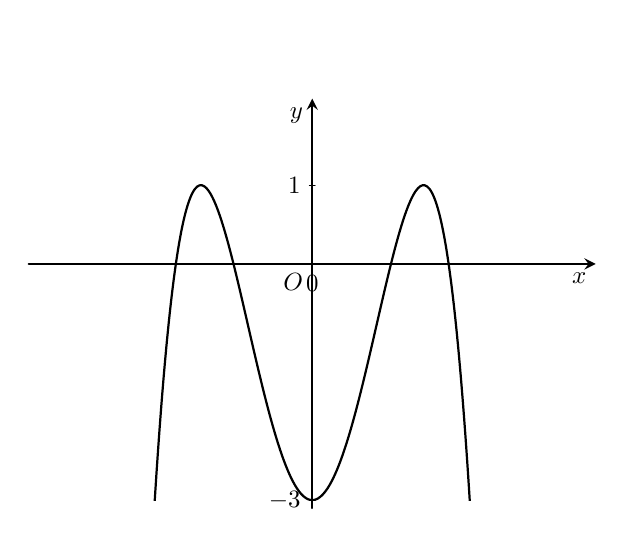
\begin{tikzpicture}[line join=round, line cap=round,>=stealth,thick]
				\tikzset{every node/.style={scale=0.9}}
				\draw[->] (-3.6,0)--(3.6,0) node[below left] {$x$};
				\draw[->] (0,-3.1)--(0,2.1) node[below left] {$y$};
				\draw (0,0) node [below left] {$O$};
				\foreach \x in {0}
				\draw[thin] (\x,1pt)--(\x,-1pt) node [below] {$\x$};
				\foreach \y in {-3,1}
				\draw[thin] (1pt,\y)--(-1pt,\y) node [left] {$\y$};
				\begin{scope}
					\clip (-3.5,-3) rectangle (3.5,3);
					\draw[samples=200,domain=-3:3,smooth,variable=\x] plot (\x,{-1*((\x)^4)+0*((\x)^3)+4*((\x)^2)+0*(\x)+-3});
				\end{scope}
			\end{tikzpicture}
		\end{center}
		Vậy để phương trình có $4 $ nghiệm phân biệt thì $-3<m<1$ 
	}
\end{ex}

\begin{ex}%[Lê Xuân Hòa]%[2D1K5-4]
	Tập tất cả các giá trị của tham số $m$ để phương trình $x^4 - 2mx^2 +2m-1  =0$ có $4$ nghiệm thực phân biệt
	\choice
	{\True $\left(\dfrac{1}{2}; +\infty\right)\setminus \left\{ 1\right\}$}
	{$(1;+\infty )$}
	{$\left(\dfrac{1}{2}; +\infty\right)$}
	{$\mathbb{R}$}
	\loigiai{
		Xét phương trình $x^4 - 2mx^2 +2m-1  =0$\quad $(1)$\\
		Đặt $t= x^2, t\le 0$\\
		Phương trình được viết lại $t^2 - 2mt +2m -1 = 0$\quad $(2)$.\\
		Để phương trình $(1)$ có $4$ nghiệm phân biệt thì phương trình $(2)$ có hai nghiệm dương phân biệt\\
		$\heva{&\Delta ' > 0\\& S>0\\& P>0}\Leftrightarrow \heva{&m^2 -2m + 1 > 0\\& 2m> 0\\& 2m-1 > 0}\Leftrightarrow \heva{& m> \dfrac{1}{2}\\& m \ne 1}\Leftrightarrow m\in \left(\dfrac{1}{2}; +\infty\right)$.
	}
\end{ex}

\begin{ex}%[Lê Xuân Hòa]%[2D1K5-4]
	Cho hàm số $y=x^4 -3x^3 - 2$. Tìm số thực $m$ dương để đường thẳng $y= m$ cắt đồ thị hàm số tại $2$ điểm phân biệt $A$, $B$ sao cho tam giác $OAB$ vuông tại $O$, trong đó $O$ là gốc tọa độ.
	\choice
	{\True $m=2$}
	{ $m=\dfrac{3}{2}$}
	{$m=3$}
	{$m=1$}
	\loigiai{
		Hoành độ giao điểm của hai đồ thị là nghiệm của phương trình $x^4 - 3x^2 - 2-m=0$\quad $(1)$.\\
		Vì $m > 0 \Rightarrow -m -2 <0$, suy ra $(1)$ luôn có hai nghiệm phân biệt thỏa\\
		$x^2 = \dfrac{3+\sqrt{4m +17}}{2}\Rightarrow x_1 = \sqrt{\dfrac{3+\sqrt{4m +17}}{2}}$ và $x_2 =-\sqrt{\dfrac{3+\sqrt{4m +17}}{2}}$.\\
		Ta có $\Delta OAB$ vuông tại $O\Leftrightarrow \overrightarrow{OA}\cdot \overrightarrow{OB}=0 \Leftrightarrow x_1x_2 +m^2 =0$.
		$\Leftrightarrow \dfrac{3+\sqrt{4m +17}}{2}=m^2 \Leftrightarrow \heva{& 2m^2 -3\le 0\\& 4m^2 -12m^2 -4m -8 = 0}\Rightarrow m =2$(do $m>0$.
	}
\end{ex}

\begin{ex}%[Lê Xuân Hòa]%[2D1K5-4]
	Đường thẳng $y=m$ cắt đồ thị hàm số $y =x^4 -x^2$ tại $4$ điểm phân biệt khi và chỉ khi
	\choice
	{\True $-\dfrac{1}{4}<m<0$}
	{$0<m<\dfrac{1}{4}$}
	{$ m>0$}
	{$ m>-\dfrac{1}{4}$}
	\loigiai{
		Tập xác định của hàm số là $\mathscr{D}=\mathbb{R}$.\\
		$y'=4x^3 -2x$; $y' = 0 \Rightarrow\heva{& x=0\\& x=\pm\dfrac{\sqrt{2}}{2}}$.\\
		Bảng biến thiên
		\begin{center}
			
\begin{tikzpicture}
				\tkzTabInit[espcl=2.5,lgt=1.5,nocadre]
				{$x$/0.7,$y'$/0.7,$y$/2.1}
				{$-\infty$,$-\frac{\sqrt{2}}{2}$,0,$\frac{\sqrt{2}}{2}$,$+\infty$}
				\tkzTabLine{,-,0,+,0,-,0,+}
				\tkzTabVar{+/$+\infty$,-/$-\frac{1}{4}$,+/$0$,-/$-\frac{1}{4}$,+/$+\infty$}
			\end{tikzpicture}
		\end{center}
		Dựa vào bảng biến thiên đường thẳng $y=m$ cắt đồ thị hàm số $y=x^2-x^2$ tại $4$ điểm phân biệt $\Leftrightarrow -\dfrac{1}{4}<m<0$.
	}
\end{ex}

\begin{ex}%[Lê Xuân Hòa]%[2D1K5-4]
	Một đường thẳng cắt đồ thị hàm số $y=x^4 -2x^2$ tại $4$ điểm phân biệt có hoành độ là $0, 1, m, n$. Tính $S=m^2 + n^2$
	\choice
	{$S=1$}
	{$S=0$}
	{\True $S=3$}
	{$S=2$}
	\loigiai{
		Tọa độ giao điểm của hai đường lần lượt là $A(0;0)$, $B(1; -1)$, $C(m; m^4-2m^2)$, $D(n; n^4 -2n^2)$.\\
		Khi đó đường thẳng qua hai điểm $A$, $B$ có phương trình $y =x$.\\
		Xét phương trình hoành độ giao điểm của $y=x^4 -2x^2$ và đường thẳng $y=x$\\
		$$x^4 -2x^2 +x =0\Leftrightarrow\hoac{&x=0\\&x=1\\&x^2+x-1=0\quad (1)}$$
		Vậy $m$, $n$ là các nghiệm của phương trình $(1)$. Với $m+n = -1; mn =-1$\\
		Khi đó $m^2 +n^2 =(m+n)^2 -2mn = 3$
	}
\end{ex}
%6
\begin{ex}%[Lê Xuân Hòa]%[2D1K5-4]
	Có bao nhiêu giá trị nguyên của $m$  để đồ thị hàm số $y= x^4 = 4x^3 +)m-2)x^2 +8x +4$  cắt trục hoành tại đúng hai điểm có hoành độ lớn hơn $1$.
	\choice
	{\True $8$}
	{$7$}
	{$5$}
	{$3$}
	\loigiai{
		Phương trình hoành độ giao điểm $x^4 -4x^3 +(m-2)x^2 +8x +4 =0$\quad $(1)$.\\
		YCBT $\Leftrightarrow (1)$ có đúng hai nghiệm lớn hơn $1$\\
		Ta có $(1) \Leftrightarrow x^4 -4x^3 +8x +4 =(2-m)x^2\Leftrightarrow 2-m = x^2 -4x +\dfrac{8}{x}+\dfrac{4}{x^2}, (x> 1).$\\
		Đây là phương trình hoành độ giao điểm của  $\mathrm{(C)} \colon y = x^2 -4x +\dfrac{8}{x}+\dfrac{4}{x^2}, (x> 1)$ với đường thẳng $y=2-m$  song song với trục hoành.\\
		Xét hàm số $x^2 -4x +\dfrac{8}{x}+\dfrac{4}{x^2}, (x> 1)$.\\
		$y' = 2x -4-\dfrac{8}{x^2}-\dfrac{8}{x^3}=\dfrac{2x^4-4x^3-8x-8}{x^2}$;\\
		$y'=0 \Rightarrow\hoac{& x=1-\sqrt{3}\text{(loại)}\\& x=1+\sqrt{3}\text{(nhận)}}$\\
		Bảng biến thiên
		\begin{center}
			
\begin{tikzpicture}
				\tkzTabInit[espcl=2.5,lgt=1.5,nocadre]
				{$x$/0.7,$y'$/0.7,$y$/2.1}
				{$1$,$1-\sqrt{3}$,$+\infty$}
				\tkzTabLine{,-,0,+}
				\tkzTabVar{+/$9$,-/$0$,+/$+\infty$}
			\end{tikzpicture}
		\end{center}
		Dựa vào bảng biến thiên, YCBT $\Leftrightarrow 0<2-m<9 \Leftrightarrow -7<m<2$.\\
		Vì $m$ nguyên nên $m \in \left\{ -6; -5; \ldots , 1\right\}$. Vậy có $8$ giá trị nguyên thỏa bài toán.
	}
\end{ex}

\begin{ex}%[Lê Xuân Hòa]%[2D1K5-4]
	Cho hàm số $f(x) = -4x^4 + 8x^2 -1$  . Có bao nhiêu giá trị nguyên dương của  m để phương trình $f(x) =m$  có đúng hai nghiệm phân biệt?
	\choice
	{$0$}
	{$2$}
	{$3$}
	{\True $1$}
	\loigiai{
		Ta có $f'(x) = -16x^3 +16x; f'(x) =0 \Leftrightarrow \Rightarrow x=0; x=\pm 1$.\\
		Bảng biến thiên
		\begin{center}
			
\begin{tikzpicture}
				\tkzTabInit[espcl=2.5,lgt=1.5,nocadre]
				{$x$/0.7,$y'$/0.7,$y$/2.1}
				{$-\infty$,$-1$,0,$1$,$+\infty$}
				\tkzTabLine{,+,0,-,0,+,0,-}
				\tkzTabVar{-/$-\infty$,+/$3$,-/$-1$,+/$3$,-/$-\infty$}
			\end{tikzpicture}
		\end{center}
		Phương trình $f(x) =m$  là phương trình hoành độ giao điểm của đồ thị hàm số  $\mathrm{(C)}: f(x) = -4x^4 + 8x^2 -1$   và đường thẳng  $d: y=m$ .
		Phương trình đã cho có $2$ nghiệm phân biệt $\Leftrightarrow$  Đường thẳng $d$  cắt đồ thị $\mathrm{(C)}$  tại hai điểm phân biệt $\Leftrightarrow \hoac{& m=3\\& m<-1}$.\\
		Vậy có $1$ giá trị nguyên dương của $m$ để phương trình $f(x) = m$ có đúng hai nghiệm phân biệt.
	}
\end{ex}

\begin{ex}%[Lê Xuân Hòa]%[2D1K5-4]
	Cho hàm số $y=x^4 +2mx^2 +m$  (với $m$  là tham số thực). Tập tất cả các giá trị của tham số $m$ để đồ thị hàm số đã cho cắt đường thẳng $y=-3$  tại bốn điểm phân biệt, trong đó có một điểm có hoành độ lớn hơn $2$  còn ba điểm kia có hoành độ nhỏ hơn $1$  , là khoảng $(a;b)$  (với  $a,b\mathbb{Q}$, $a,b$ là phân số tối giản). Khi đó,  $15ab$ nhận giá trị nào sau đây?
	\choice
	{$-63$}
	{$63$}
	{\True $95$}
	{$-95$}
	\loigiai{
		Xét phương trình hoành độ giao điểm $x^4 +2mx^2 +m =-3$  . Đặt  $x^2 =t, t> 0$ . Khi đó phương trình trở thành  $t^2 +2mt +m +3 =0$, \quad $(1)$   và đặt $f(t) = t^2 +2mt +m +3$ .
		Để đồ thị hàm số cắt đường thẳng $y=-3$  tại $4$  điểm phân biệt thì phương trình  $(1)$ có hai nghiệm thỏa mãn $0<t_1<t_2$  và khi đó hoành độ bốn giao điểm là $-\sqrt{t_2}<-\sqrt{t_1}<\sqrt{t_1}<\sqrt{t_2}$ ..
		Do đó, từ điều kiện của bài toán suy ra  $\heva{&\sqrt{t_2}\\&\sqrt{t_1}<1}$ hay $0<t_1 < 1< 4< t_2$  .
		Điều này xảy ra khi và chỉ khi  $\heva{& f(0) > 0\\& f(1) <0\\& f(4) < 0}\Leftrightarrow \heva{&m + 3 > 0\\& 3m +4 < 0\\&9m +19 < 0}\Leftrightarrow -3 < m < -\dfrac{19}{9}$  .
		Vậy $a= -3$, $b=-\dfrac{19}{9}$ nên $15ab = 95$ .
		
	}
\end{ex}
%9
\begin{ex}%[Lê Xuân Hòa]%[2D1K5-4]
	Đường thẳng $y=m^2$  cắt đồ thị hàm số $y=x^4 -x^2 -10$  tại hai điểm phân biệt  $A$, $B$ sao cho tam giác  $OAB$ vuông ($O$  là gốc tọa độ). Mệnh đề nào sau đây đúng?
	\choice
	{$m^2\in (5;7)$}
	{$m^2\in (3;5)$}
	{\True $m^2\in (1;3)$}
	{$m^2\in (0;1)$}
	\loigiai{
		Ta có $y' = 4x^3 -2x$; $y' = 0\Rightarrow x = 0; x=\pm\dfrac{1}{\sqrt{2}}$\\
		Bảng biến thiên
		\begin{center}
			
\begin{tikzpicture}
				\tkzTabInit[espcl=2.5,lgt=1.5,nocadre]
				{$x$/0.7,$y'$/0.7,$y$/2.1}
				{$-\infty$,$-0.71$,0,$0.71$,$+\infty$}
				\tkzTabLine{,-,0,+,0,-,0,+}
				\tkzTabVar{+/$+\infty$,-/$-10.25$,+/$-10$,-/$-10.25$,+/$+\infty$}
			\end{tikzpicture}
		\end{center}
		Dựa vào bảng biến thiên, ta thấy đường thẳng  $y=m^2 > 0$ luôn phía trên trục hoành nên nó luôn cắt đồ thị hàm số tại hai điểm phân biệt  $A$, $B$.
		Gọi $A\left( \sqrt{a}; m^2\right)$  và $B\left( -\sqrt{a}; m^2\right)$  là giao điểm của hai đồ thị đã cho, với  $a> 0$. Ta có 
		\begin{itemize}
			\item $A\in\mathrm{(C)} \Rightarrow a^2- a - 10 =0$\quad $(1)$
			\item Tam giác $OAB$ cân tại $O$ nên tam giác $OAB$ vuông tại $O \Leftrightarrow \overrightarrow{OA}\cdot\overrightarrow{OB}=0\Leftrightarrow m^4 =a$\quad $(2)$.\\
			Từ $(1)$ và $(2)$ ta có $\Leftrightarrow m^8 - m^4 -m^2 -10 =0 \Leftrightarrow t^4 - t^2 -t -10 =0$, với $t=m^2 > 0$\\
			$\Leftrightarrow (t-2)(t^3 +2t^2 +3t +5) = 0\Leftrightarrow t= 2 \Leftrightarrow m^2 =2\in (1;3)$.
		\end{itemize}
	}
\end{ex}

\begin{ex}%[Lê Xuân Hòa]%[2D1K5-4]
	\immini{ Cho hàm số $y= x^4-2x^2-3$  có đồ thị như hình vẽ bên dưới. Với giá trị nào của  $m$ thì phương trình $x^4-2x^2-3 = 2m-4$  có $2$  nghiệm phân biệt.
	}
	{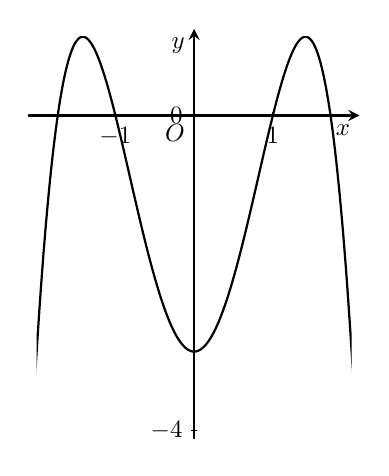
\begin{tikzpicture}[line join=round, line cap=round,>=stealth,thick]
			\tikzset{every node/.style={scale=0.9}}
			\draw[->] (-2.1,0)--(2.1,0) node[below left] {$x$};
			\draw[->] (0,-4.1)--(0,1.1) node[below left] {$y$};
			\draw (0,0) node [below left] {$O$};
			\foreach \x in {-1,1}
			\draw[thin] (\x,1pt)--(\x,-1pt) node [below] {$\x$};
			\foreach \y in {-4,0}
			\draw[thin] (1pt,\y)--(-1pt,\y) node [left] {$\y$};
			\begin{scope}
				\clip (-2,-4) rectangle (2,1);
				\draw[samples=200,domain=-3:3,smooth,variable=\x] plot (\x,{-1*((\x)^4)+0*((\x)^3)+4*((\x)^2)+0*(\x)+-3});
				\draw[samples=200,domain=-3:3,smooth,variable=\x] plot (\x,{1*((\x)^4)+0*((\x)^3)+-2*((\x)^2)+0*(\x)+3});
			\end{scope}
	\end{tikzpicture}}
	\choice
	{$\hoac{&m<0\\&m=\dfrac{1}{2}}$}
	{$m\le \dfrac{1}{2}$}
	{$0< m<\dfrac{1}{2}$}
	{$\hoac{&m=0\\&m>\dfrac{1}{2}}$}
	\loigiai{
		Dựa vào đồ thị, ta có $\hoac{&2m-4=0\\&2m-4>-3}\Leftrightarrow \hoac{&m=0\\&m>\dfrac{1}{2}}$
	}
\end{ex}
%11
\begin{ex}%[Lê Xuân Hòa]%[2D1K5-4]
	Tìm tất cả các giá trị của tham số  $m$ để phương trình $-x^4 + 2x^2 + 3 +2m =0$  có $4$  nghiệm phân biệt.
	\choice
	{$-2\le m\le =\dfrac{3}{2}$}
	{$-\dfrac{3}{2}<m<2$}
	{\True $-2<m<=\dfrac{3}{2}$}
	{$3<m<4$}
	\loigiai{
		Ta có $-x^4 + 2x^2 + 3 +2m =0\Leftrightarrow x^4 - 2x^2-3 =2m$\\
		Lập bảng biến thiên của hàm số $y=x^4 - 2x^2 -3$
		\begin{center}
			
\begin{tikzpicture}
				\tkzTabInit[espcl=2.5,lgt=1.5,nocadre]
				{$x$/0.7,$y'$/0.7,$y$/2.1}
				{$-\infty$,$-1$,0,$1$,$+\infty$}
				\tkzTabLine{,-,0,+,0,-,0,+}
				\tkzTabVar{+/$+\infty$,-/$-4$,+/$-3$,-/$-4$,+/$+\infty$}
			\end{tikzpicture}
		\end{center}
		Dựa vào bảng biến thiên, YCBT $\Leftrightarrow -4<2m<-3\Leftrightarrow -2< m <-\dfrac{3}{2}$.
	}
\end{ex}

\begin{ex}%[Lê Xuân Hòa]%[2D1K5-4]
	Tất cả các giá trị thực của tham số  $m$, để đồ thị hàm số $y=x^4 - 2(2-m)x^2 + m^2 -2m -2$  không cắt trục hoành.
	\choice
	{$m\ge \sqrt{3}+ 1$}
	{$m< 3$}
	{\True $ m> \sqrt{3}+1$}
	{$m> 3$}
	\loigiai{
		Xét phương trình hoành độ giao điểm $x^4 -2(2-m)x^2 + m^2 -2m -2 = 0$ \quad $(1)$\\
		Đặt $t= x^2 \ge 0$. Phương trình $(1)$ trở thành $t^2 -2(2-m)t +m^2 -2m -2 =0$\quad $(2)$\\
		Đồ thị hàm số không cắt trục hoành $\Leftrightarrow (1)$ vô nghiệm $\Leftrightarrow (2)$ vô nghiệm hoặc có nghiệm âm\\
		Hay $\hoac{& \Delta ' = -2m + 6 < 0\\&\heva{&\Delta ' =2m +6 \ge 0\\& 2-m <0\\& m^2 -2m -2 > 0}}\Leftrightarrow \hoac{&m > 3\\&\heva{&m\le 3\\&m>2\\&\hoac{& m>1 + \sqrt{3}\\& m <1-\sqrt{3}}}}\Leftrightarrow \hoac{&m > 3\\& 1+\sqrt{3} < m \le 3}\Leftrightarrow m > 1+\sqrt{3}$.
	}
\end{ex}

\begin{ex}%[Lê Xuân Hòa]%[2D1K5-4]
	Tìm tất cả các giá trị của tham số  $m$ để đồ thị hàm số $y=(m+1)x^4 -2(2m -3)x^2 + 6m +5$ cắt trục hoành tại $4$ điểm phân biệt có các hoành độ $x_1, x_2, x_3, x_4$ thỏa mãn $x_1< x_2<x_3 < 1 <x_4$  thỏa mãn  
	\choice
	{$m\in\left( -1; -\dfrac{5}{6}\right)$}
	{$m\in (-3; -1)$}
	{$m\in (-3; 1)$}
	{\True $m\in (-4; -1)$}
	\loigiai{
		Phương trình hoành độ giao điểm của đồ thị hàm số và trục hoành là
		$$y=(m+1)x^4 -2(2m -3)x^2 + 6m +5,\quad (1)$$
		Đặt $t=x^2 \ge 0$ pt trở thành  
		$y=(m+1)t^2 -2(2m -3)t + 6m +5$,\quad $(2)$
		Để pt (1) có 4 nghiệm phân biệt thì pt (2) phải có 2 nghiệm dương phân biệt
		Hay   $\heva{&m+1\ne 0\\& \Delta ' > 0\\&t_1t_2 > 0\\& t_1 + t_2 > 0  }\heva{&m\ne -1\\& (2m-3)^2 -(m+1)(6m +5) > 0\\& \dfrac{6m +5}{m +1}\\&\dfrac{2m -3}{m +1}> 0  } \Leftrightarrow\heva{& m\ne -1\\& \dfrac{-23-\sqrt{561}}{4}\\& m <-1; m >-\dfrac{5}{6}\\& m < -1; m > \dfrac{3}{2} }\quad (1)$\\
		Để pt (1) có 4 nghiệm thỏa mãn  $x_1< x_2<x_3 < 1< x_4$ 
		thì pt (2) phải có 2 nghiệm thỏa  $0< t_1< 1< t_2$\\
		$\Leftrightarrow\heva{&t_1 - 1 < 0\\& t_2 -1 > 0 }\Leftrightarrow \heva{&(t_1-1)(t_2-1) < 0} \Leftrightarrow t_1t_2 - (t_1 t_2) + 1 < 0$\\
		$\Leftrightarrow \dfrac{6m +5}{m +1}-\dfrac{2(2m -3)}{m +1}+1 < 0\Leftrightarrow \dfrac{3m +12}{m+1}< 0 \Leftrightarrow -4 < m < -1$.\\
		Kết hợp $(1)$ ta có $m\in (-4; -1)$.
	}
\end{ex}

\begin{ex}%[Lê Xuân Hòa]%[2D1K5-4]
	Cho hàm số  $y= x^4 -(3m +2)x^2 + 3m$ có đồ thị là $\mathrm{(C_m)}$ . Tìm $m$  để đường thẳng $d\colon y = -1$  cắt đồ thị  $\mathrm{(C_m)}$ tại $4$ điểm phân biệt đều có hoành độ nhỏ hơn $2$.
	\choice
	{\True $=\dfrac{1}{3} < m < 1$ và $  m \ne 0$}
	{$-\dfrac{1}{2}< m < 1$ và $m\ne 0$}
	{$-\dfrac{1}{2}< m < \dfrac{1}{2}$ và $m\ne 0$}
	{$-\dfrac{1}{3}< m < 1$ và $m\ne 0$}
	\loigiai{
		Phương trình hoành độ giao điểm của $\mathrm{(C_m)}$ và đường thẳng $d$  là   $x^4 -(3m +2)x^2 + 3m+ 1 = 0$ \quad $(2)$\\
		Đặt $t= x^2 \ge 0$  phương trình trở thành \\
		$t^4 -(3m +2)t^2 + 3m+ 1 =0$\quad $(2)$  $\Leftrightarrow \hoac{&t = 1\\& t = 3m +1}$
		Đường thẳng $d$  cắt đồ thị $\mathrm{(C_m)}$  tại $4$  điểm phân biệt đều có hoành độ nhỏ hơn $2$  khi và chỉ khi phương trình  có hai nghiệm dương phân biệt $t_1, t_2$   thỏa mãn  $0< t_1 < t_2 < 4$.
		
		$\Leftrightarrow\heva{&3m +1 \ne 1\\& 0< 3m +1 < 4} \Leftrightarrow \heva{&m\ne 0\\& -\dfrac{1}{3}< m < 1.}$
	}
\end{ex}

\begin{ex}%[Lê Xuân Hòa]%[2D1K5-4]
	Tìm tất cả các giá trị thực của $m$  để phương trình $|x^4 - 2x^2 -3| = 2m -1$   có đúng $6$  nghiệm thực phân biệt
	\choice
	{$1< m < \dfrac{3}{2}$}
	{$4< m <5$}
	{$3< m < 4$}
	{\True $2< m < \dfrac{5}{2}$}
	\loigiai{
		Xét hàm số $g(x) = x^4 - 2x^2 - 3$, có tập xác định $\mathscr{D} = \mathbb{R}$\\
		$g'(x) = 4x^3 - 4x$, $g'(x) = 0 \Rightarrow \hoac{&x=0\\& x= \pm 1  }$\\
		Bảng biến thiên 
		\begin{center}
			
\begin{tikzpicture}
				\tkzTabInit[espcl=2.5,lgt=1.5,nocadre]
				{$x$/0.7,$y'$/0.7,$y$/2.1}
				{$-\infty$,$-1$,0,$1$,$+\infty$}
				\tkzTabLine{,-,0,+,0,-,0,+}
				\tkzTabVar{+/$+\infty$,-/$-4$,+/$-3$,-/$-4$,+/$+\infty$}
			\end{tikzpicture}
		\end{center}
		Suy ra bảng biến thiên của hàm số $y= |x^4 - 2x^2 -3| $ 
		\begin{center}
			
\begin{tikzpicture}
				\tkzTabInit[espcl=2.5,lgt=1.5,nocadre]
				{$x$/0.7,$y$/2.1}
				{$-\infty$,$-\sqrt{3}$,$-1$,0,$1$,$\sqrt{3}$,$+\infty$}
				%\tkzTabLine{,-,0,+,0,+,0,-,0,+}
				\tkzTabVar{+/$+\infty$,-/$0$,+/$4$,-/$-3$,+/$4$,-/$0$,+/$+\infty$}
			\end{tikzpicture}
		\end{center}
		YCBT $\Leftrightarrow 3 < 2m -1 < 4\Leftrightarrow 2 < m \dfrac{5}{2}$
	}
\end{ex}
\Closesolutionfile{ans}
	\indapan{10}{ans/CD6/Muc_7_8}